\documentclass[UTF8]{article}

\usepackage[zihao=5]{ctex}		%字号设置
\usepackage[a4paper]{geometry}	%页面设置
\geometry{left=1.5cm,right=1.5cm,top=2cm,bottom=4.3cm} %GPA+=4.3
\usepackage{graphicx} 			%插入并编辑图片
\usepackage{siunitx}			%更好看的物理单位(手打其实更快些)
\usepackage{chemfig}
\usepackage{amsthm}
\usepackage{subfigure}
\usepackage{fancyhdr}			%设置页眉页脚
\usepackage{lmodern}			%一种编码字体
\usepackage{amsmath}			%数学公式扩展
\usepackage{amssymb}
\usepackage{multicol}
\usepackage{fontspec}
\usepackage{float}
\numberwithin{figure}{subsection}
\numberwithin{table}{subsection}
\usepackage{threeparttable}		%三线表宏包1
\usepackage{booktabs}			%三线表宏包2
\usepackage{listings} % 引入宏包
\usepackage{xcolor}   % 可以用来定义颜色
\usepackage{hyperref}

% 定义MATLAB代码的显示风格
\lstset{language=Matlab,
	breaklines=true,
	basicstyle=\ttfamily,
	keywordstyle=\color{blue},
	commentstyle=\color{green},
	stringstyle=\color{red},
	showstringspaces=false,
}

\graphicspath{{figure/}}		%将报告中需要的图片储存于此

\pagestyle{fancy}				%设置页眉页脚
\setlength{\headheight}{70pt}
\lhead{
\includegraphics[scale=0.7]{logo.PNG}}
%需要将学校的logo名命并放入figures文件夹中
\chead{}
\rhead{}

\newtheorem{theorem}{\indent 定理}[subsection]
\newtheorem{lemma}[theorem]{\indent 引理}
\newtheorem{proposition}[theorem]{\indent 命题}
\newtheorem{corollary}[theorem]{\indent 推论}
\newtheorem{definition}{\indent 定义}[subsection]
\newtheorem{example}{\indent 例}[subsection]
\newtheorem{remark}{\indent 注}[subsection]
\newenvironment{solution}{\begin{proof}[\indent\bf 解]}{\end{proof}}
\renewcommand{\proofname}{\indent\bf 证明}

\begin{document}
\begin{center}
    \LARGE{\textbf{基于MATLAB可视化常见电磁学模型}}

    \vspace*{0.2cm}
    \normalsize{陈昕琪    PB22111711 \qquad \\ 2023年12月6日}
\end{center}
\normalsize
\noindent \textbf{摘要:}电磁场概念和空间分布具有抽象性,使得课程中理解计算较为困难。本文基于MATLAB对电磁学中的常见模型进行了可视化研究。通过课堂上已学的知识进行公式推导,并对常见的理想化电磁学模型进行可视化处理,包括电场强度,电势,电场线,磁感应强度等的可视化。本文所展示的电磁学模型可视化结果丰富直观,通过逐点取值,公式运算等方法,使得抽象的概念更加直观具体,方便初学者理解。

\noindent \textbf{关键词:}MATLAB;电磁学;电场强度;电势;磁感应强度;
\begin{multicols}{2}
    \section{引言}
    \par 电磁学作为物理学的一个基础分支,在现代科技发展中扮演着至关重要的角色。从日常生活中的电器设备到航空航天领域的高精尖技术,无不涉及电磁理论的应用。然而,电磁学的概念往往涉及复杂的物理现象和数学表达,这对于学习和研究者而言是一大挑战。在这种背景下,可视化工具的引入显得尤为重要,它能够帮助我们更直观地理解电磁场的分布和变化规律。
    \par MATLAB(Matrix Laboratory的缩写)是一款强大的数学计算软件,广泛用于工程计算、数据分析、算法开发以及图形绘制等领域。通过MATLAB,用户可以方便地进行矢量场的计算、电磁波的传播模拟以及频率响应的分析等。
    \par 在电磁学的可视化实现上,MATLAB提供了多种方法。例如,使用其二维和三维绘图功能,可以直观地展示电场和磁场的分布情况;通过偏微分方程(PDE)工具箱,可以求解各种电磁问题的数值解,并将结果以图形的形式呈现出来;此外,MATLAB的仿真功能还可以帮助研究人员模拟电磁波在不同介质中的传播过程,以及在复杂结构中的散射、折射现象。
    \par 本文旨在介绍MATLAB在电磁学模型可视化中的应用,并通过几个典型的电磁学问题展示如何利用MATLAB进行模型的建立、求解和可视化,以期为电磁学的教学和科研提供一定的参考和帮助。
    
    \section{可视化模型呈现}
    \par 以下内容将分为6个部分,从常见的电磁学模型入手,计算电场,电势,磁感应强度等物理量。
    \par 仅展示核心代码,所有MATLAB文件已传到GitHub网站,欢迎大家学习交流。(文末已放置链接)
    \begin{remark}为了方便处理数据,以下MATLAB程序未计算出精确数字,而是在已知常量的基础上计算,仅反应物理量变化规律。
    \end{remark}
    \subsection{模拟电偶极子场强分布}
    \subsubsection{问题描述}
    \par 利用matlab编程计算电偶极子的电势和电场强度的大小和方向,并绘制图像进行可视化。
    \subsubsection{公式推导}
    \par 电偶极子由两个等量但相反符号的点电荷组成,这里设定正电荷位于(x, y) = (1,0)位置,负电荷位于(x, y) = (-1, 0)位置。
    \par 设电偶极子电荷量大小为q。则电偶极子存在的平面内一点的电势推导公式如下:
    $$r_1=\sqrt{{x+1}^2+y^2}$$
    $$r_2=\sqrt{{x-1}^2+y^2}$$
    $$U=\frac{-q}{r_1}+\frac{q}{r_2}$$
    \par 其中,(x,y)表示平面内点的位置。
    \par 电场是电势的负梯度,因此电场的分量可以表示为:
    $$E=-\nabla U$$
    \subsubsection{代码解释}
    \par 首先用MATLAB的linspace和meshgrid函数初始化变量和构建网格。
    \par 然后根据已推导出的公式计算$r_1$,$r_2$。并且构建电势表达式:其中,$Phi$ 根据电势公式计算由两个点电荷产生的电势。(这里设q=1)
    \begin{lstlisting}
    q=1;
    xm=2.5;
    ym=2;
    x=linspace(-xm,xm);
    y=linspace(-ym,ym);
    [X,Y]=meshgrid(x,y);
    r1=sqrt((X+1).^2+Y.^2);
    r2=sqrt((X-1).^2+Y.^2);
    Phi=-q./r1+q./r2;
    \end{lstlisting}
    \par 计算出电势后,进行绘图操作。使用 contour 函数绘制电势的等高线(虚线)。
    \begin{lstlisting}
    u=-4:0.5:4;
    figure
    contour(X,Y,Phi,u,'--');
    hold on
    \end{lstlisting}
    \par 使用gradient函数计算电势场的梯度,得到电场的分量(EX,EY)。重复绘图操作。用 streamline 函数绘制电场线。电场线的起点是通过极坐标转换来确定的,围绕每个电荷画圆弧形状的电场线。
    \begin{lstlisting}
    [EX1,EY1]=gradient(-Phi,x(1),y(1));
    %构造stratline函数的起点
    dth1=20;
    th1=(dth1:dth1:180-dth1)*pi/180;
    r0=0.1;
    %构造左侧电场线起点x1,y1
    x1=r0*cos(th1)-1;
    y1=r0*sin(th1);
    %运用streamline函数进行电场线绘制
    streamline(X,Y,EX1,EY1,x1,y1);
    streamline(X,-Y,EX1,-EY1,x1,-y1);
    hold on 
    %右边
    [EX2,EY2]=gradient(-Phi,x(100),y(100));
    dth2=20;
    th2=(180-dth2:-dth2:dth2)*pi/180;
    x2=r0*cos(th2)+1;
    y2=r0*sin(th2);
    streamline(X,Y,EX2,EY2,x2,y2);
    streamline(X,-Y,EX2,-EY2,x2,-y2);
    axis equal tight
    \end{lstlisting}
    \par 除此之外,还可以将二维平面图转化为三维立体图更有助于理解,在电磁学课本中讲解电偶极子的部分,配有类似的图,在这里通过matlab实现简单还原。
    \par 将电势作为z坐标绘图。
    \begin{lstlisting}
    r1=sqrt((X+1).^2+Y.^2);
    r2=sqrt((X-1).^2+Y.^2);
    Phi=-q./r1+q./r2;
    %运用mesh函数绘制Phi,X,Y三维图
    mesh(X,Y,Phi)
    hold on 
    \end{lstlisting}
	\par 当然也可以据此画出电场强度的三维图,在这里不多赘述。
    \subsubsection{结果展示}
    \begin{figure}[H]
    	\centering
    	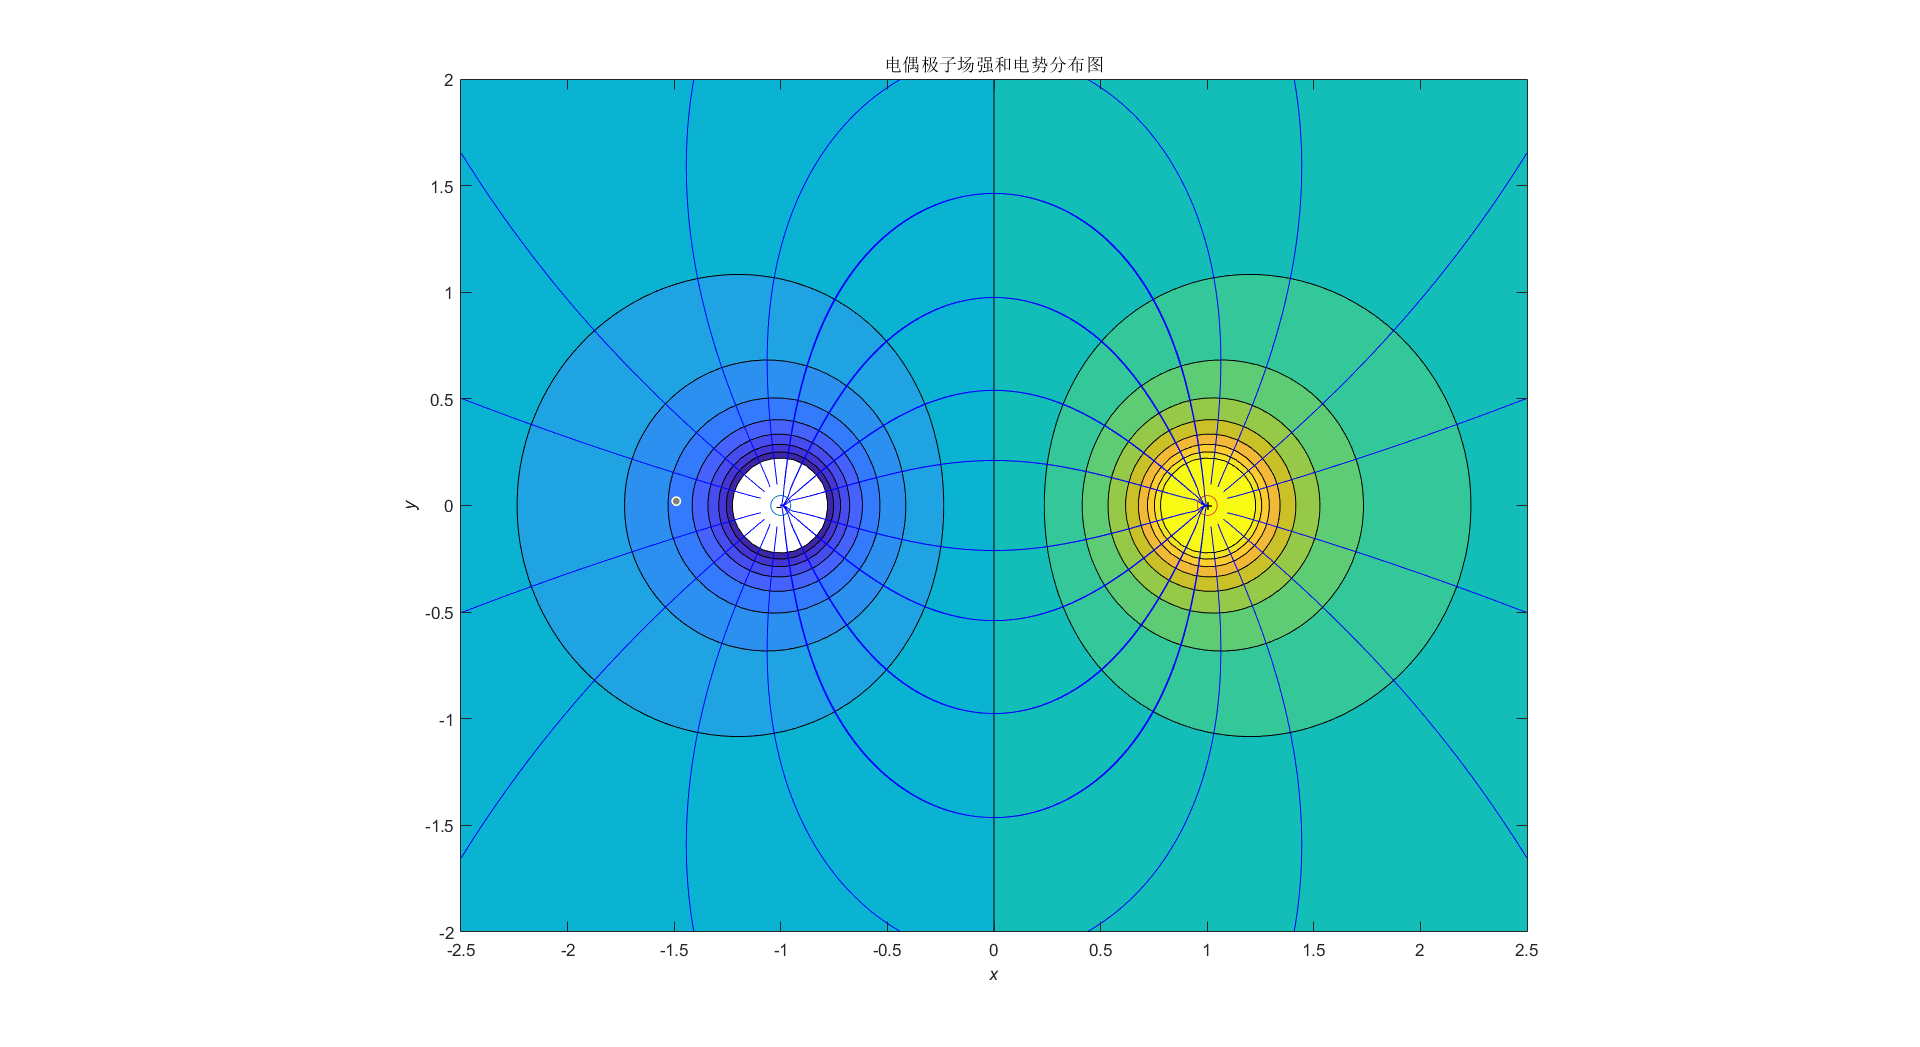
\includegraphics[scale=0.15]{电偶极子场强分布.png}
    	\caption{二维平面电偶极子场强分布}
    \end{figure}
	\begin{figure}[H]
		\centering
		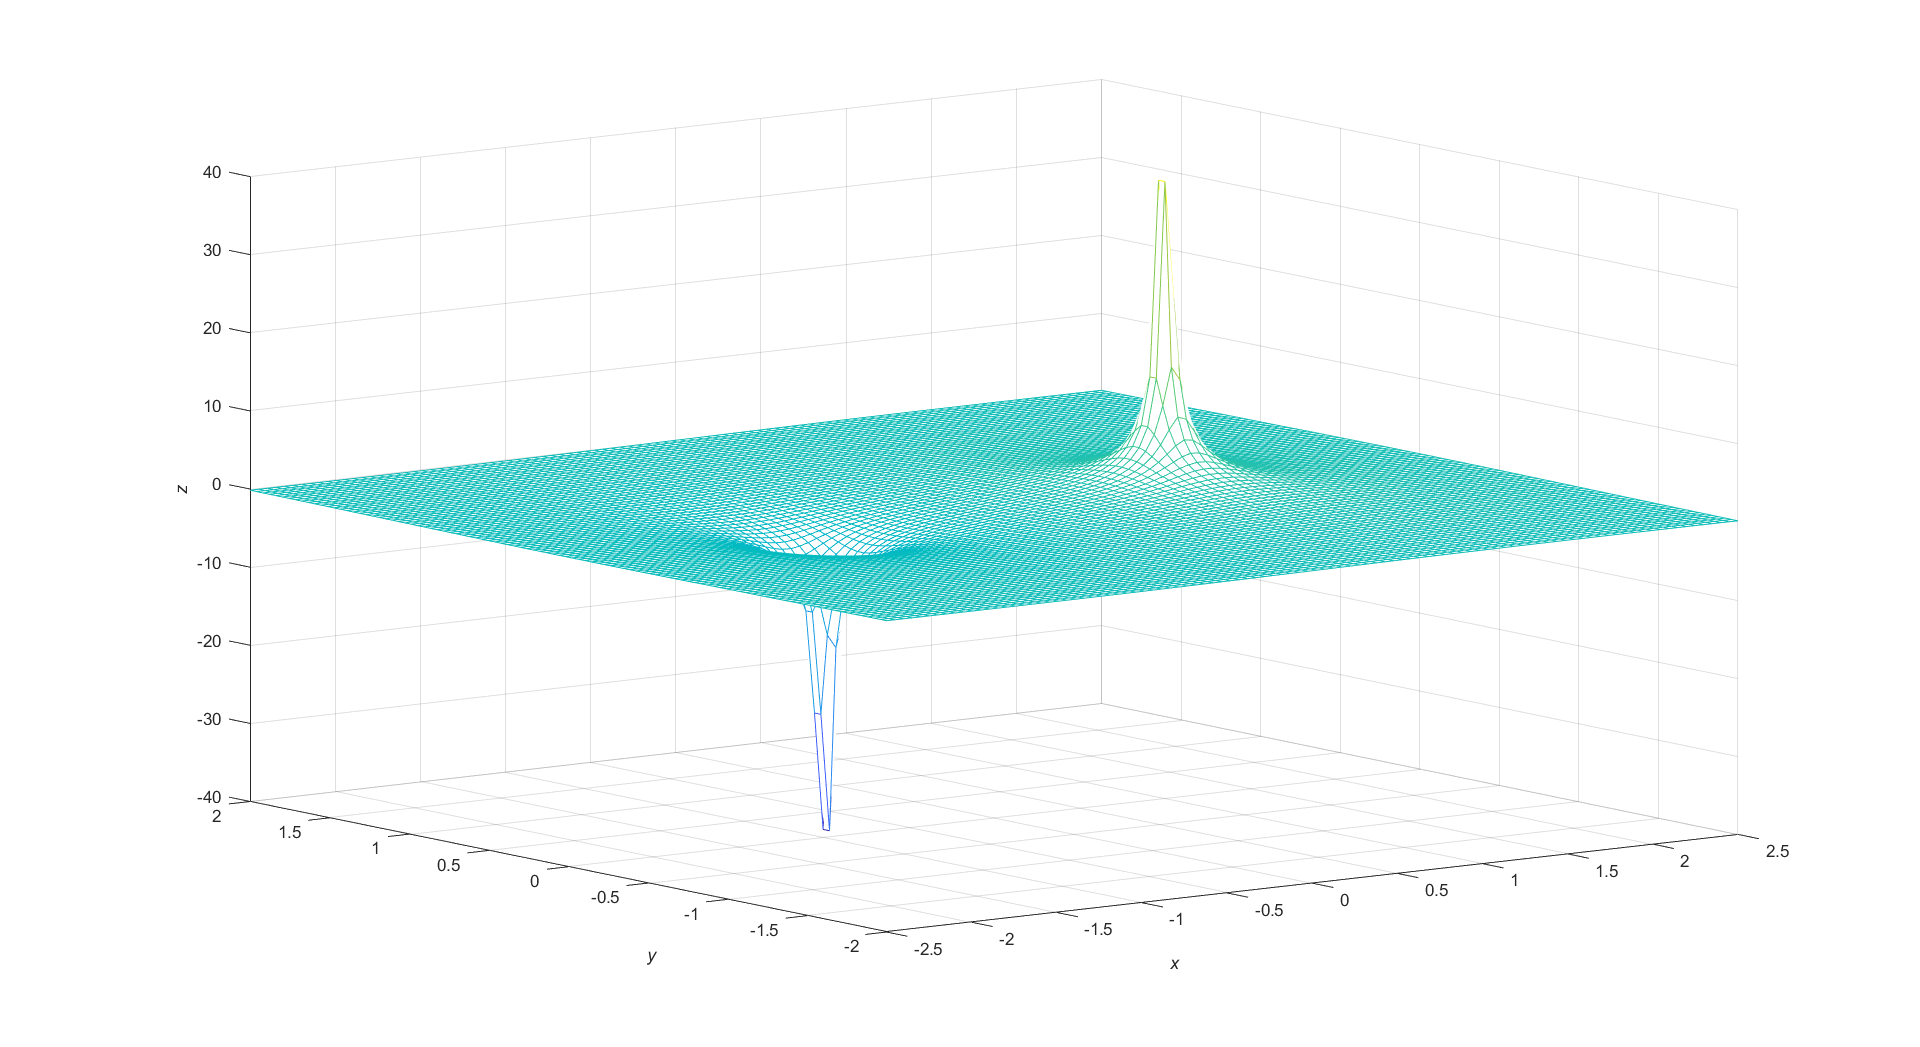
\includegraphics[scale=0.15]{立体图.png}
		\caption{三维电偶极子电势分布}
	\end{figure}
	\subsection{求点电荷的电场强度和电势}
	\subsubsection{问题描述}
	\par 用Matlab仿真点电荷电场强度和电势。
	\subsubsection{公式推导}
	\par 设点电荷电量为Q,根据公式可以得出距离点电荷为r处点电荷产生的的电场强度公式和电势公式如下:
	$$E = \frac{kQ}{r^2}$$
	$$U = \frac{kQ}{r}$$
	\subsubsection{代码解释}
	\par 首先对参数初始化并根据已推导出的公式直接计算出$\frac{E}{E_0}$,$\frac{U}{U_0}$。
	\par 然后初始化图形,并绘制点电荷的电场强度和电势图。
	\begin{lstlisting}
    clear %清除变量
    r0 = 2.5;%最大相对距离
    r = 0.2:0.05:r0;%距离向量
    e = 1./r.^2;%电场强度
    u = 1./r;%电势
    figure %创建图形窗扣款
    plot(r,e,r,u,'--','LineWidth',3);%画电场强度和电势曲线
    grid on%加网格
    axis([0,r0,0,5]);%曲线范围
	\end{lstlisting}
	\subsubsection{结果展示}
	\begin{figure}[H]
		\centering
		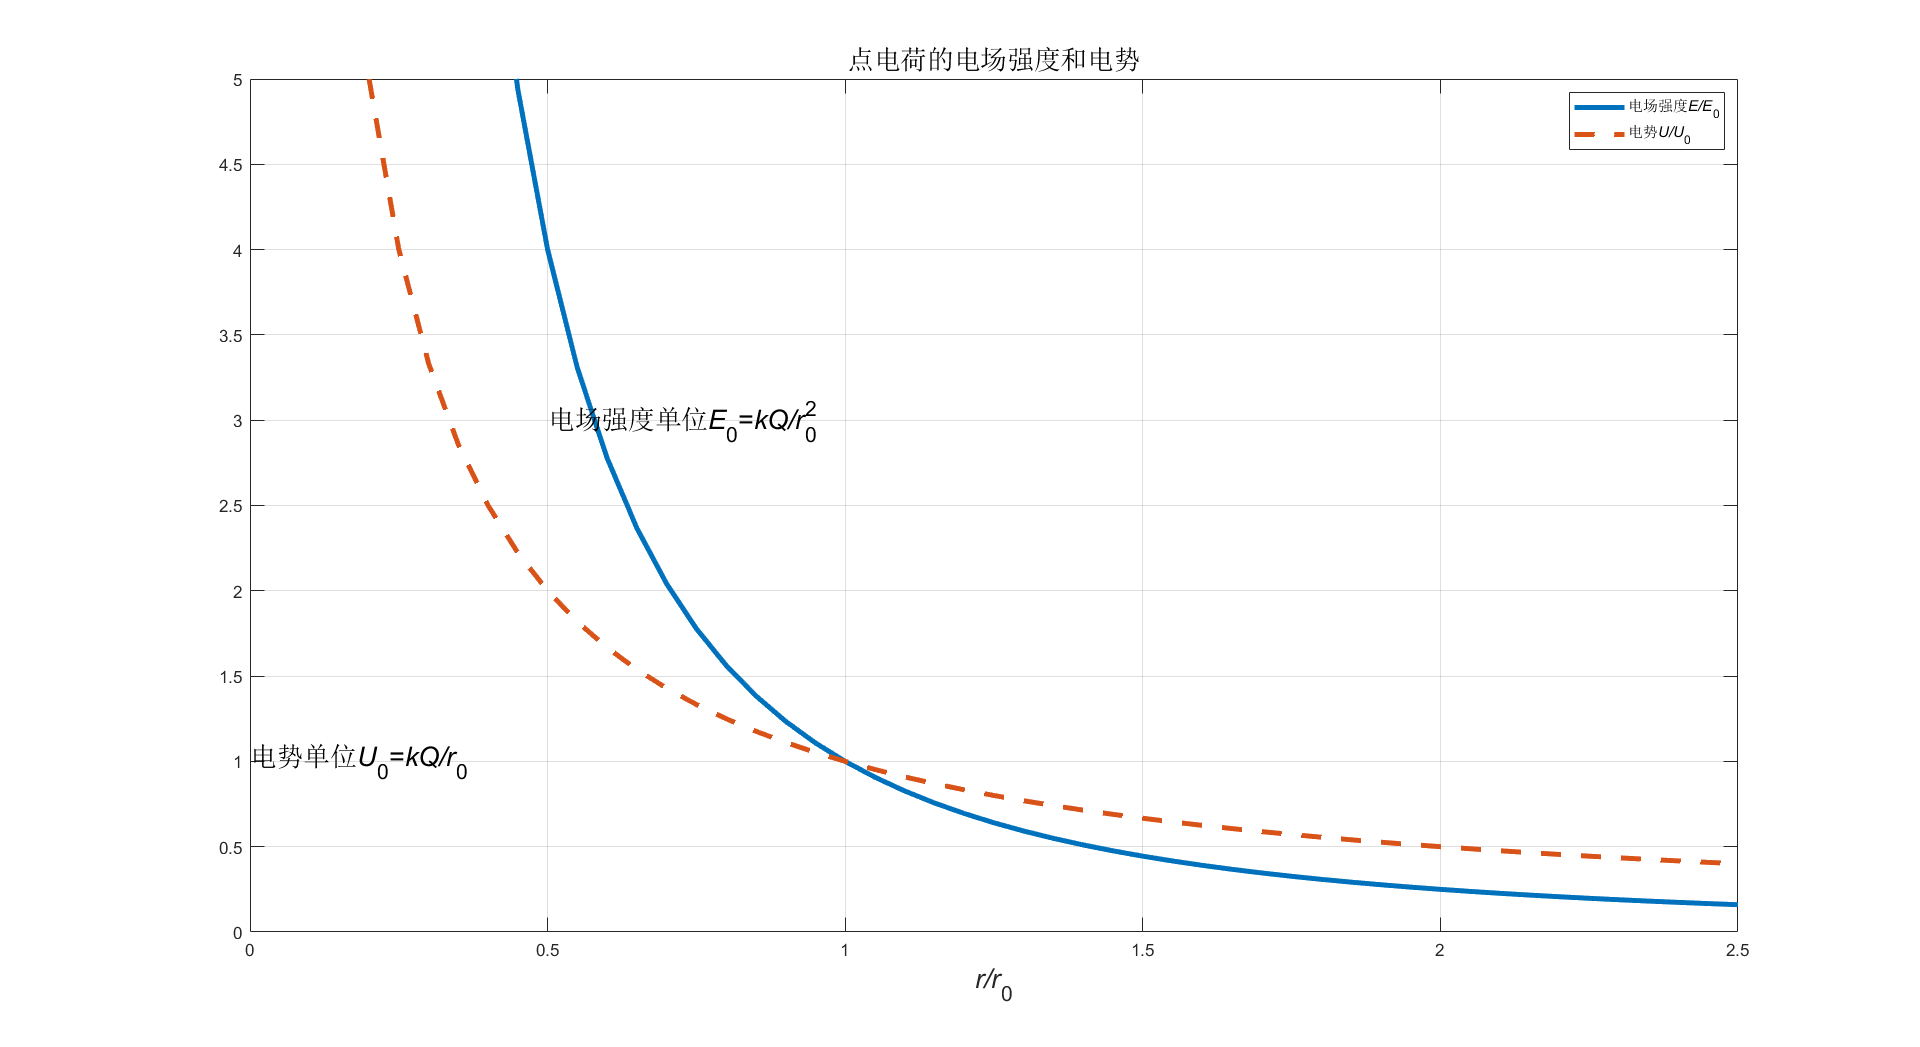
\includegraphics[scale=0.15]{点电荷电场强度和电势.png}
		\caption{点电荷的电场强度和电势}
	\end{figure}
    \subsection{均匀带电圆环、圆盘在轴线上的电场仿真}
    \subsubsection{问题描述}
    \par 带电圆环和带电圆盘是电磁学中常见的物理模型。用Matlab仿真均匀带电圆环和均匀带电圆盘轴线上的电场强度和电势。
    \subsubsection{公式推导}
    \par 1. 均匀带电圆环的轴线电场强度和电势:
    \par 考虑一个半径为 \( R \) 的均匀带电圆环,其总电荷量为 \( Q \)。设圆环在 \( z \) 轴上某点 \( P \)(距离圆心 \( O \) 的距离为 \( z \))产生的电场强度和电势。
    \par 首先,将圆环分割成微小的电荷元素 \( dq \),每个电荷元素在 \( P \) 点产生的电场强度 \( d\mathbf{E} \) 可以分解为垂直于轴线的分量 \( dE_\perp \) 和平行于轴线的分量 \( dE_{||} \)。由对称性,垂直分量在 \( P \) 点相互抵消,只有平行分量贡献总电场强度。
    \par 电荷元素 \( dq \) 在 \( P \) 点产生的电场强度的平行分量为:
    \[ dE_{||} = \frac{1}{4\pi\epsilon_0} \frac{dq}{R^2+z^2} \cos\theta, \]
    其中 \( \cos\theta = \frac{z}{\sqrt{R^2+z^2}} \),因此:
    \[ dE_{||} = \frac{1}{4\pi\epsilon_0} \frac{z \, dq}{(R^2+z^2)^{3/2}}. \]
    \par 积分 \( dq \) 得到总电场强度 \( E \):
    \[ E = \int dE_{||} = \frac{1}{4\pi\epsilon_0} \frac{z}{(R^2+z^2)^{3/2}} \int dq. \]
    \par 由于圆环上的总电荷为 \( Q \),则:
    \[ E = \frac{kQz}{(R^2+z^2)^{3/2}}. \]
    \par 对于电势 \( V \),由于电场沿轴线是保守场,我们可以计算 \( dq \) 在 \( P \) 点产生的电势 \( dV \):
    \[ dV = \frac{kQ}{4\pi\epsilon_0} \frac{dq}{\sqrt{R^2+z^2}}. \]
    \par 积分得到总电势 \( V \):
    \[ V = \int dV = \frac{1}{4\pi\epsilon_0} \int \frac{dq}{\sqrt{R^2+z^2}} = \frac{kQ}{\sqrt{R^2+z^2}} \]
    \par 2. 均匀带电圆盘的轴线电场强度和电势
    \par 现在考虑一个半径为 \( R \) 的均匀带电圆盘,总电荷量为 \( Q \),面密度 \( \sigma = \frac{Q}{\pi R^2} \)。与圆环类似,我们考虑圆盘上微元 \( dA = 2\pi r \, dr \) 上的电荷 \( dq = \sigma dA = 2\pi \sigma r \, dr \),在轴线上 \( z \) 处产生的电场强度的分量 \( dE_{||} \)。
    
    \[ dE_{||} = \frac{1}{4\pi\epsilon_0} \frac{dq}{r^2+z^2} \cos\theta = \frac{1}{4\pi\epsilon_0} \frac{2\pi \sigma r \, dr}{(r^2+z^2)} \frac{z}{\sqrt{r^2+z^2}}. \]
    
    \par 积分 \( r \) 从 0 到 \( R \) 得到总电场强度 \( E \):
    \[ E = \frac{\sigma z}{2\epsilon_0} \int_0^R \frac{r \, dr}{(r^2+z^2)^{3/2}}. \]
    
    \par 通过变量代换和积分,我们得到:
    \[ E = \frac{\sigma}{2\epsilon_0} \left(1 - \frac{z}{\sqrt{R^2+z^2}}\right) = \frac{z}{|z|} \frac{2kQ}{R^2} (1-\frac{|z|}{\sqrt{z^2+R^2}}). \]
    
    \par 电势 \( V \),从无穷远处到 \( z \) 处的积分给出:
    \[ V = \frac{\sigma}{2\epsilon_0} \left(\sqrt{R^2+z^2} - z\right) = \frac{2kQ}{R^2} (\sqrt{z^2+a^2}-|z|). \]
    
    \subsubsection{代码解释}
    \par 首先初始化变量,并根据公式计算出带电圆环的轴线处的电场强度和电势。
    \begin{remark}
    	在实际操作中发现引入k值往往难以计算,因此在这里设q=1,r=1,并求出$\frac{U}{k}$的值,也可以能反应物理量变化规律。
    \end{remark}
	\begin{lstlisting}
    u1=Q./sqrt(z.^2+a^2);             % 圆环在轴线上的电势 U/k
    e1=Q*z./((z.^2+a^2).^1.5);        % 圆环在轴线上的电场强度 E/k
    u2=2*Q*(sqrt(z.^2+a^2)-abs(z));   % 圆盘在轴线上的电势 U/k
    e2=2*Q*sign(z).*(1-abs(z)./sqrt(1+z.^2))/a^2; % 圆盘在轴线上的电场强度 E/k
	\end{lstlisting}
    \par 这里的 u1 和 e1 是根据均匀带电圆环的电势和电场公式计算得到的,而 u2 和 e2 则是根据均匀带电圆盘的电势和电场公式计算得到的。
    \par 在得出结果后,绘制图形。使用 figure 和 plot 函数来创建图形窗口并绘制电势和电场强度的图像设置曲线宽度,添加图例,如绘制圆环轴线上电势分布代码如下:
    \begin{lstlisting}
    figure
    plot(z,u1, 'LineWidth' ,3)
    legend('圆环的电势\itU/k','2') 
    grid on
    axis([-zm,zm,-10,10])
    fs=16;
    title('均匀带电圆环在轴线上的电势','FontSize',fs)
    xlabel('与带电圆环中心的距离z','FontSize',fs)%显示x坐标
    \end{lstlisting}
    \par 重复绘图过程,代码中的其他 figure 块用于绘制圆环电场强度、圆盘电势和圆盘电场强度的图像。
    \subsubsection{结果展示}
    \begin{figure}[H]
    	\centering
    	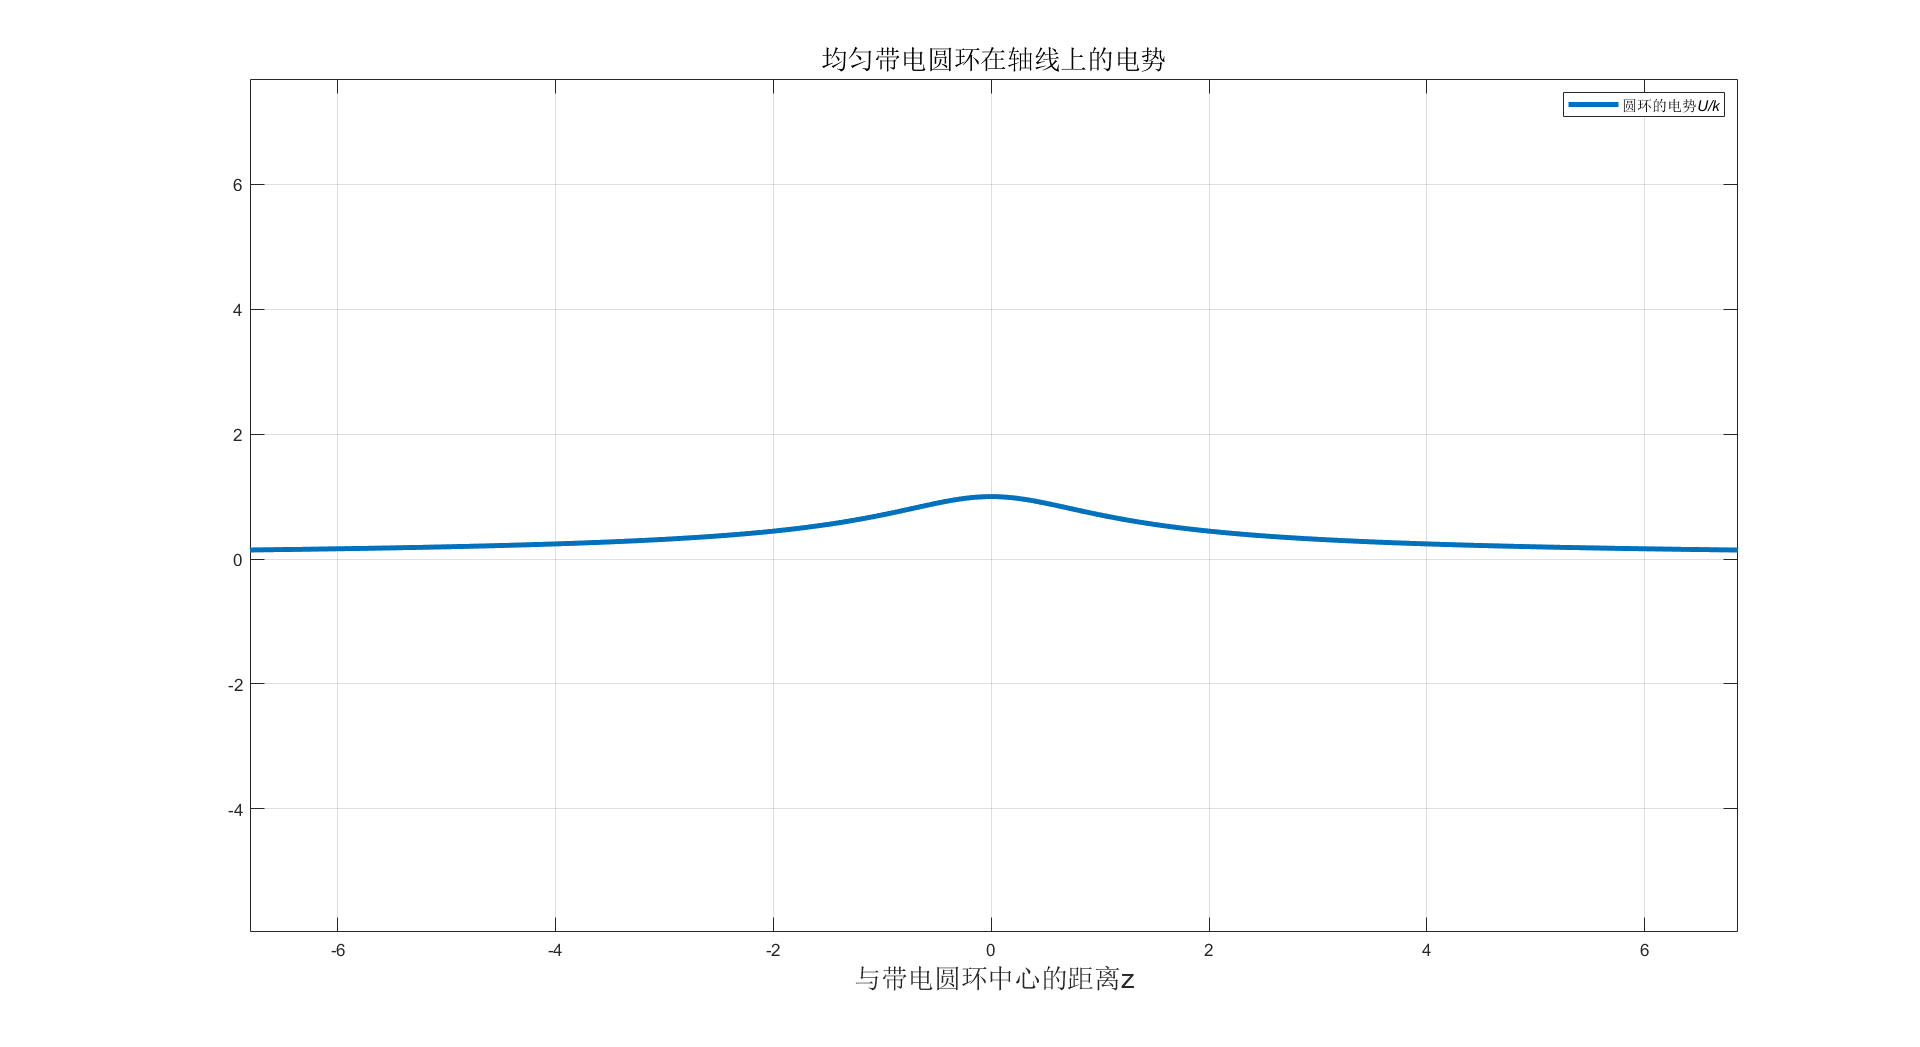
\includegraphics[scale=0.15]{圆环电势.png}
    	\caption{均匀带电圆环在轴线上的电势}
    \end{figure}
	\begin{figure}[H]
		\centering
		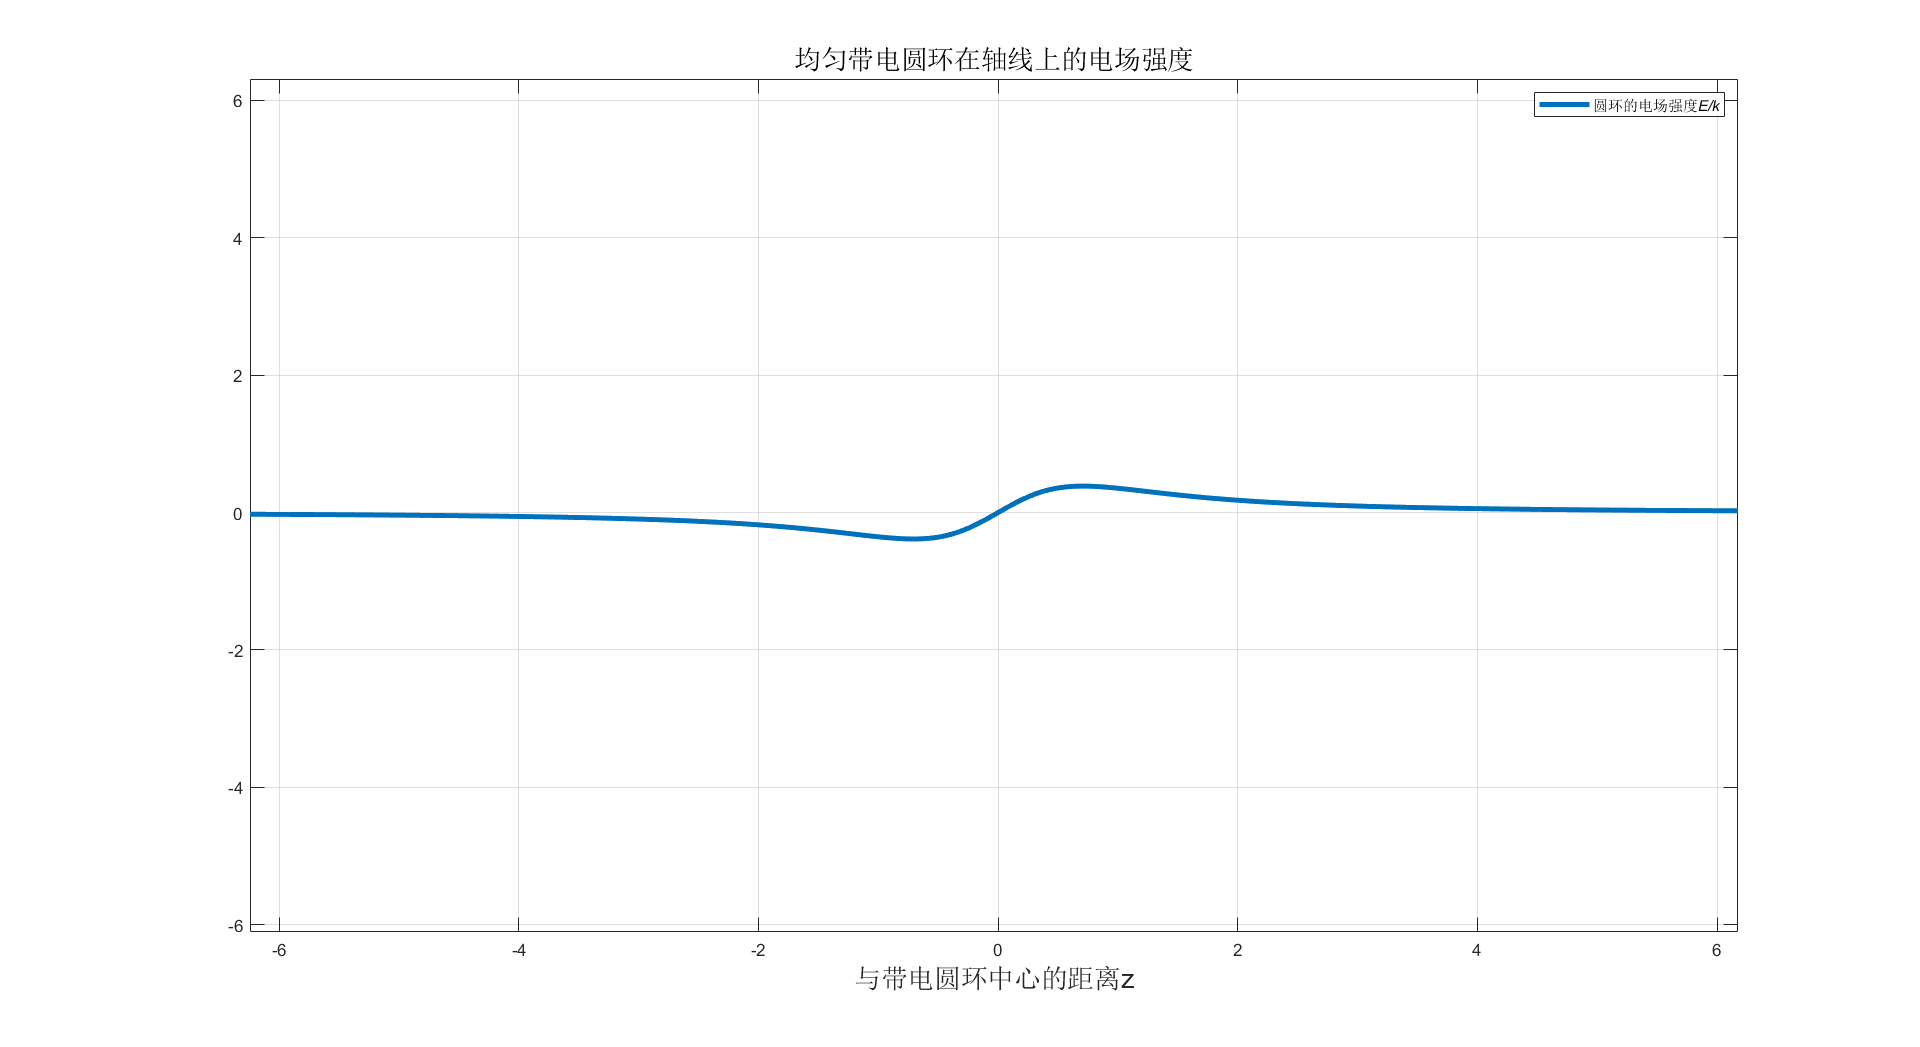
\includegraphics[scale=0.15]{圆环场强.png}
		\caption{均匀带电圆环在轴线上的电场强度}
	\end{figure}
	\begin{figure}[H]
		\centering
		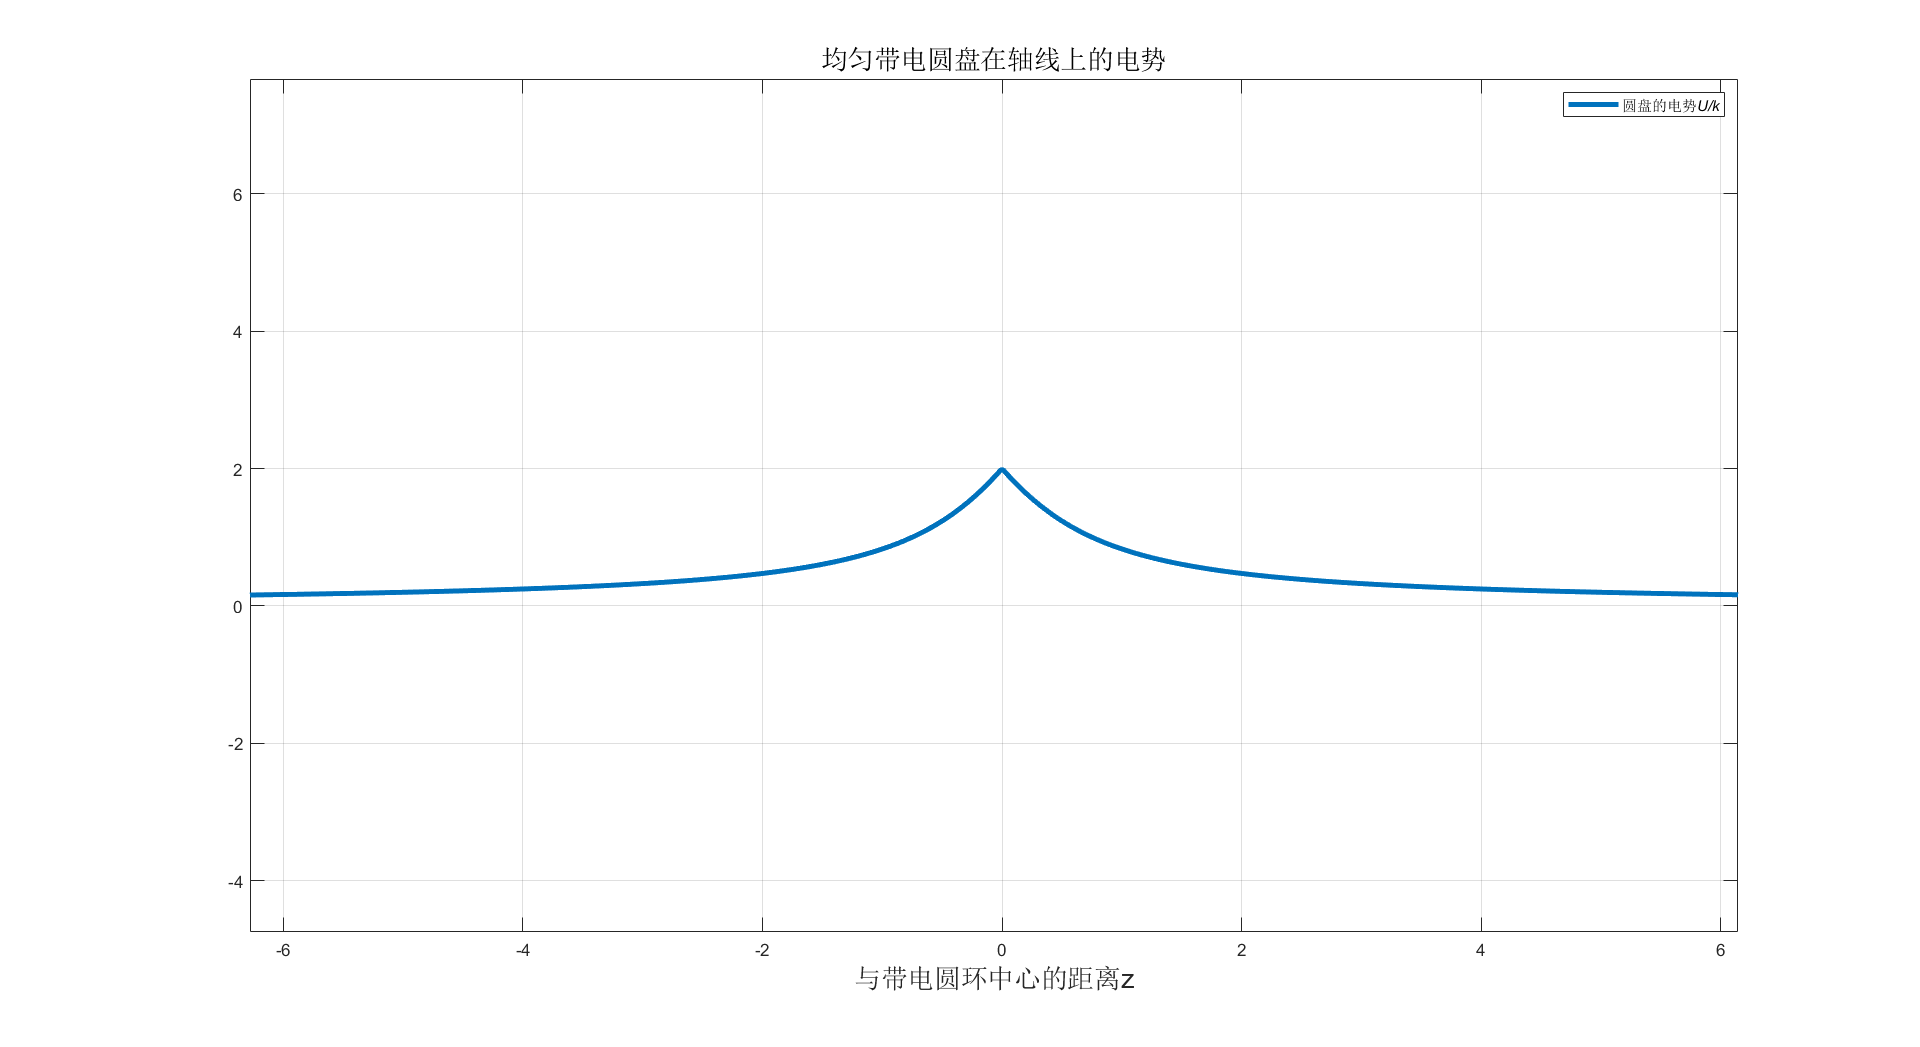
\includegraphics[scale=0.15]{圆盘电势.png}
		\caption{均匀带电圆盘在轴线上的电势}
	\end{figure}
	\begin{figure}[H]
		\centering
		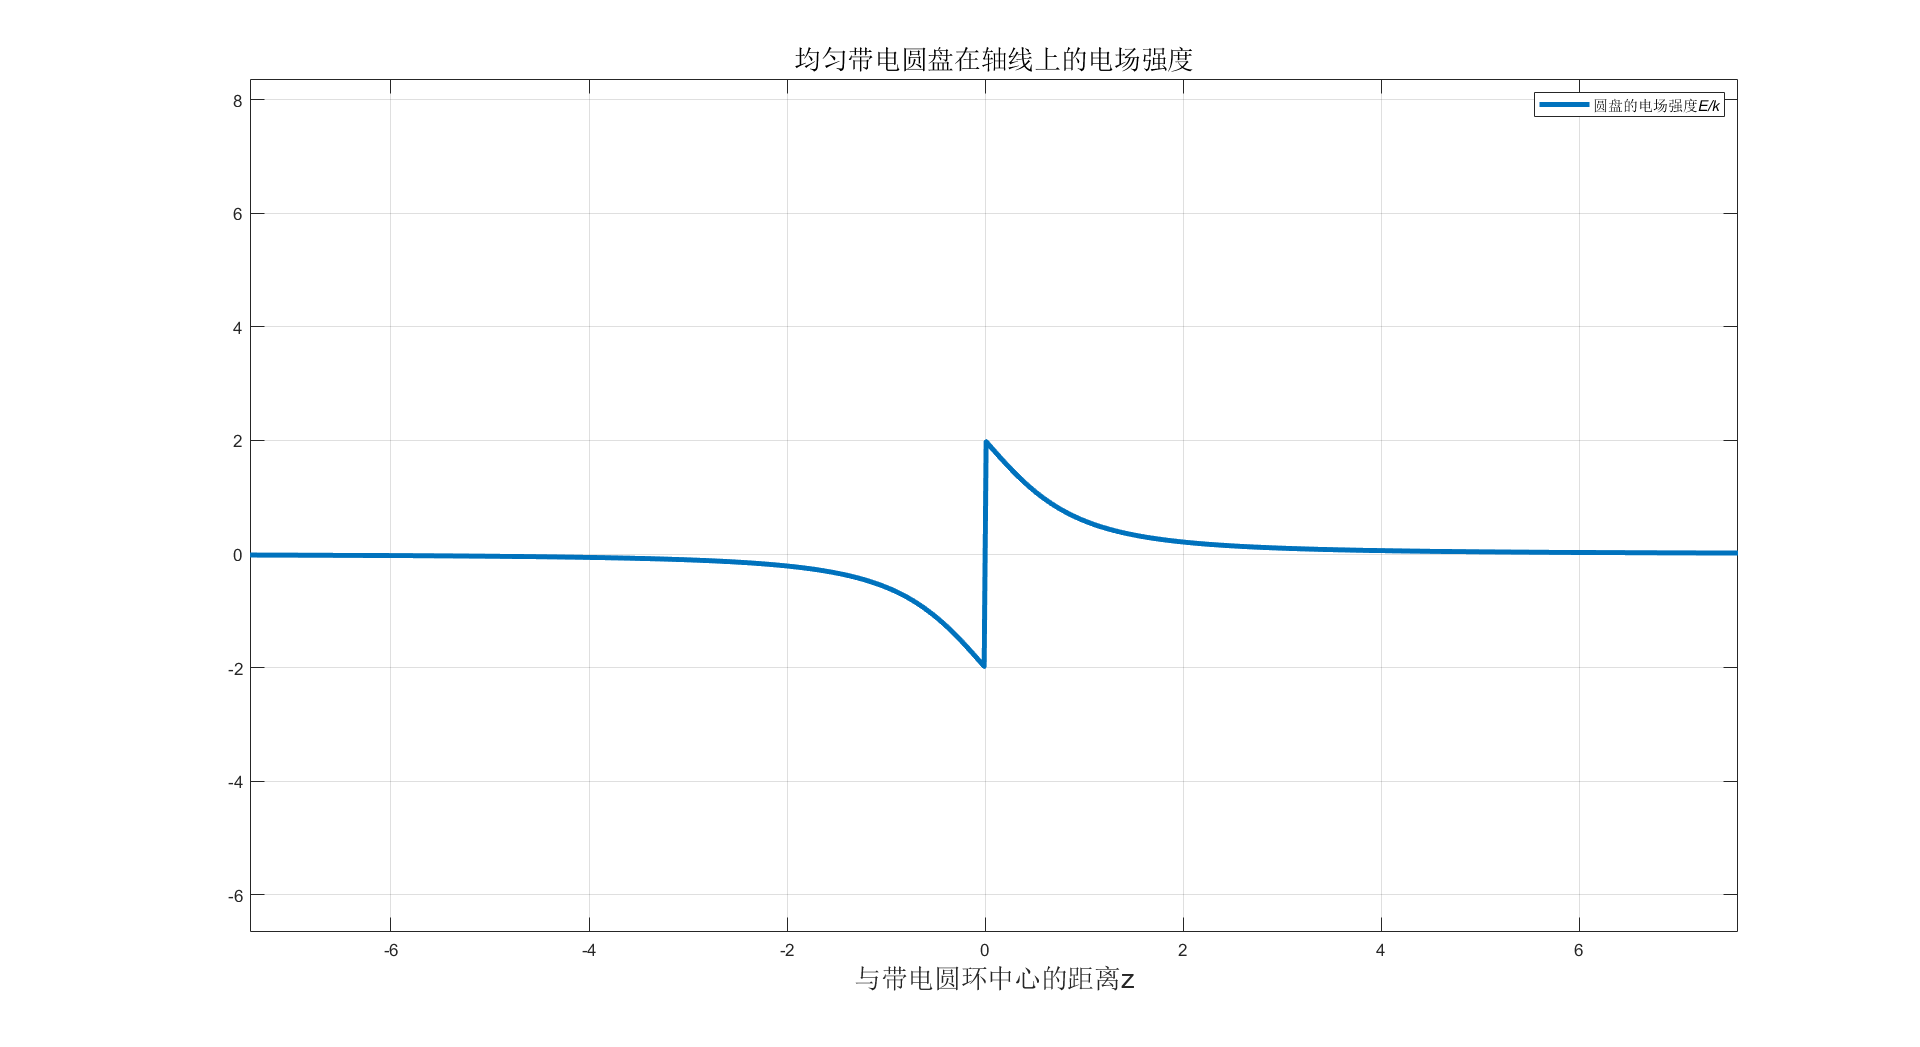
\includegraphics[scale=0.15]{圆盘场强.png}
		\caption{均匀带电圆盘在轴线上的电场强度}
	\end{figure}
	\subsection{求均匀带电球壳的电场}
	\subsubsection{问题描述}
	\par 一均匀带电球壳,内部是空腔,球壳内外半径分别为R0和R,带电量为Q,用MATLAB仿真,求空间各点的电场强度和电势,对于不同的球壳厚度,电场强度和电势随距离变化的规律是什么?
	\subsubsection{公式推导}
	\par 对于一个内部为空腔的均匀带电球壳,其内外半径分别为 $R_0$ 和 $R$,带电量为 $Q$,可以将空间分为三个区域来讨论电场强度和电势:
	
	\begin{enumerate}
		\item 球壳内部空腔区域($r < R_0$);
		\item 球壳本身区域($R_0 \leq r \leq R$);
		\item 球壳外部区域($r > R$)。
	\end{enumerate}
	
	电场强度 $E$:
	
	\par 球壳内部空腔区域($r < R_0$):
	\par 由于电荷只分布在球壳上,因此根据高斯定律,在球壳内部的电场强度为零。即:
	\[ E = 0 \quad  \quad r < R_0 \]
	
	球壳本身区域($R_0 \leq r \leq R$):
	由于电荷均匀分布在球壳的厚度上,我们可以通过积分来计算某一点 $r$ 处的电场强度。设球壳的体积电荷密度为 $\rho$,则有 
	\[ \rho = \frac{Q}{\frac{4}{3}\pi (R^3 - R_0^3)} \]
	考虑到对称性,我们选择以球心为中心的球面作为高斯面。对于 $R_0 \leq r \leq R$ 区域内任意点,电场强度 $E$ 可以通过以下高斯定律公式计算:
	\[ E \cdot 4\pi r^2 = \frac{Q_{\text{enclosed}}}{\varepsilon_0} \]
	其中 $Q_{\text{enclosed}}$ 是高斯面内包含的电荷量,$\varepsilon_0$ 是真空的电容率。由于电荷均匀分布,$Q_{\text{enclosed}}$ 可以通过体积电荷密度乘以高斯面内的体积来计算:
	\[ Q_{\text{enclosed}} = \rho \cdot \frac{4}{3}\pi (r^3 - R_0^3) \]
	代入 $\rho$ 和 $Q_{\text{enclosed}}$ 的表达式,我们可以得到 $r$ 处的电场强度 $E$:
	\[ E = \frac{\rho}{3\varepsilon_0}(r^3 - R_0^3) \cdot \frac{1}{r^2} \]
	\[ E = \frac{Q}{4\pi\varepsilon_0(R^3 - R_0^3)} \cdot \frac{r - R_0^3/r^2}{3} \]
	
	球壳外部区域($r > R$):
	球壳外部的电场强度可以看作是由位于球心的点电荷 $Q$ 所产生的电场。因此,电场强度 $E$ 为:
	\[ E = \frac{Q}{4\pi\varepsilon_0 r^2} \quad  \quad r > R \]
	
	电势 $V$:
	
	电势 $V$ 可以通过电场强度 $E$ 积分得到。通常情况下,我们会选择无穷远处的电势为零作为参考点。
	
	球壳内部空腔区域($r < R_0$):
	由于内部电场强度为零,电势在整个空腔内部是常数。我们可以从 $r = R$ 开始积分,因为在这个位置电势是已知的。因此,电势 $V$ 为:
	\[ V = \frac{Q}{4\pi\varepsilon_0 R} \quad  \quad r < R_0 \]
	
	球壳本身区域($R_0 \leq r \leq R$):
	在球壳内部,电势 $V$ 需要通过积分电场强度 $E$ 来计算:
	\[ V(r) = -\int_{R}^{r} E \, dr + V(R) \]
	由于电场强度 $E$ 在球壳内部随着 $r$ 变化,我们需要将上面得到的 $E$ 表达式代入并积分。
	
	球壳外部区域($r > R$):
	球壳外部的电势 $V$ 同样可以通过积分电场强度 $E$ 来计算:
	\[ V(r) = -\int_{\infty}^{r} E \, dr = -\left[-\frac{Q}{4\pi\varepsilon_0 r}\right]_{\infty}^{r} \]
	\[ V(r) = \frac{Q}{4\pi\varepsilon_0 r} \quad  \quad r > R \]
	\par 即
	\begin{align}
		\left\{
		\begin{aligned}
			E&=0,U=\frac{3kQ(R+R_0)}{2(R^2+RR_0+R_0^2)}  (r\leq R_0) \\
			E&=\frac{kQ}{R^3-R_0^3} (r-\frac{R_0^3}{r^3}),\\
			U&=\frac{kQ}{2(R^3-R_0^3)} (3R^3-r^3-\frac{2R_0^3}{r}) (R_0\leq r\leq R)\\
			E&=\frac{kQ}{r^2},U=\frac{kQ}{r} (R\leq r)
		\end{aligned}   
		\right.
	\end{align}
	\subsubsection{代码解释}
	\par 首先初始化变量。
	\begin{remark}
		\par 本代码分为三个区域计算电场强度和电势。
		\par 1. 球壳内部(rA):电场强度为0,电势为常数。
		\par 2. 球壳上(rB):电场强度和电势按照球壳上的物理公式计算。
		\par 3. 球壳外部(rC):电场强度和电势按照点电荷的物理公式计算。
	\end{remark}
	\par 需要用户键入球壳的内半径与外半径之比,根据推导出的公式,计算出电场强度和电势。
	\begin{lstlisting}
    clear
    r0 = input('请输入内半径与外半径之比(大于等于0小于等于1);');
    rm = 4;
    dr = 0.01;
    rA = 0:dr:r0;
    uA = ones(size(rA))*3/2*(1+r0)/(1+r0+r0^2);
    eA = -diff(uA)/dr;
    rB = r0:dr:1;
    uB = (3-rB.^2-2*r0^3./rB)/2/(1-r0^3);
    eB = -diff(uB)/dr;
    rC = 1:dr:rm;
    uC = 1./rC;
    eC = -diff(uC)/dr;
	\end{lstlisting}
	\par 使用subplot函数来创建两个子图,第一个子图绘制电场强度,第二个子图绘制电势。设置添加位宽,网格线等,并添加一些文本信息,方便理解。
	\subsubsection{结果展示}
	\begin{figure}[H]
		\centering
		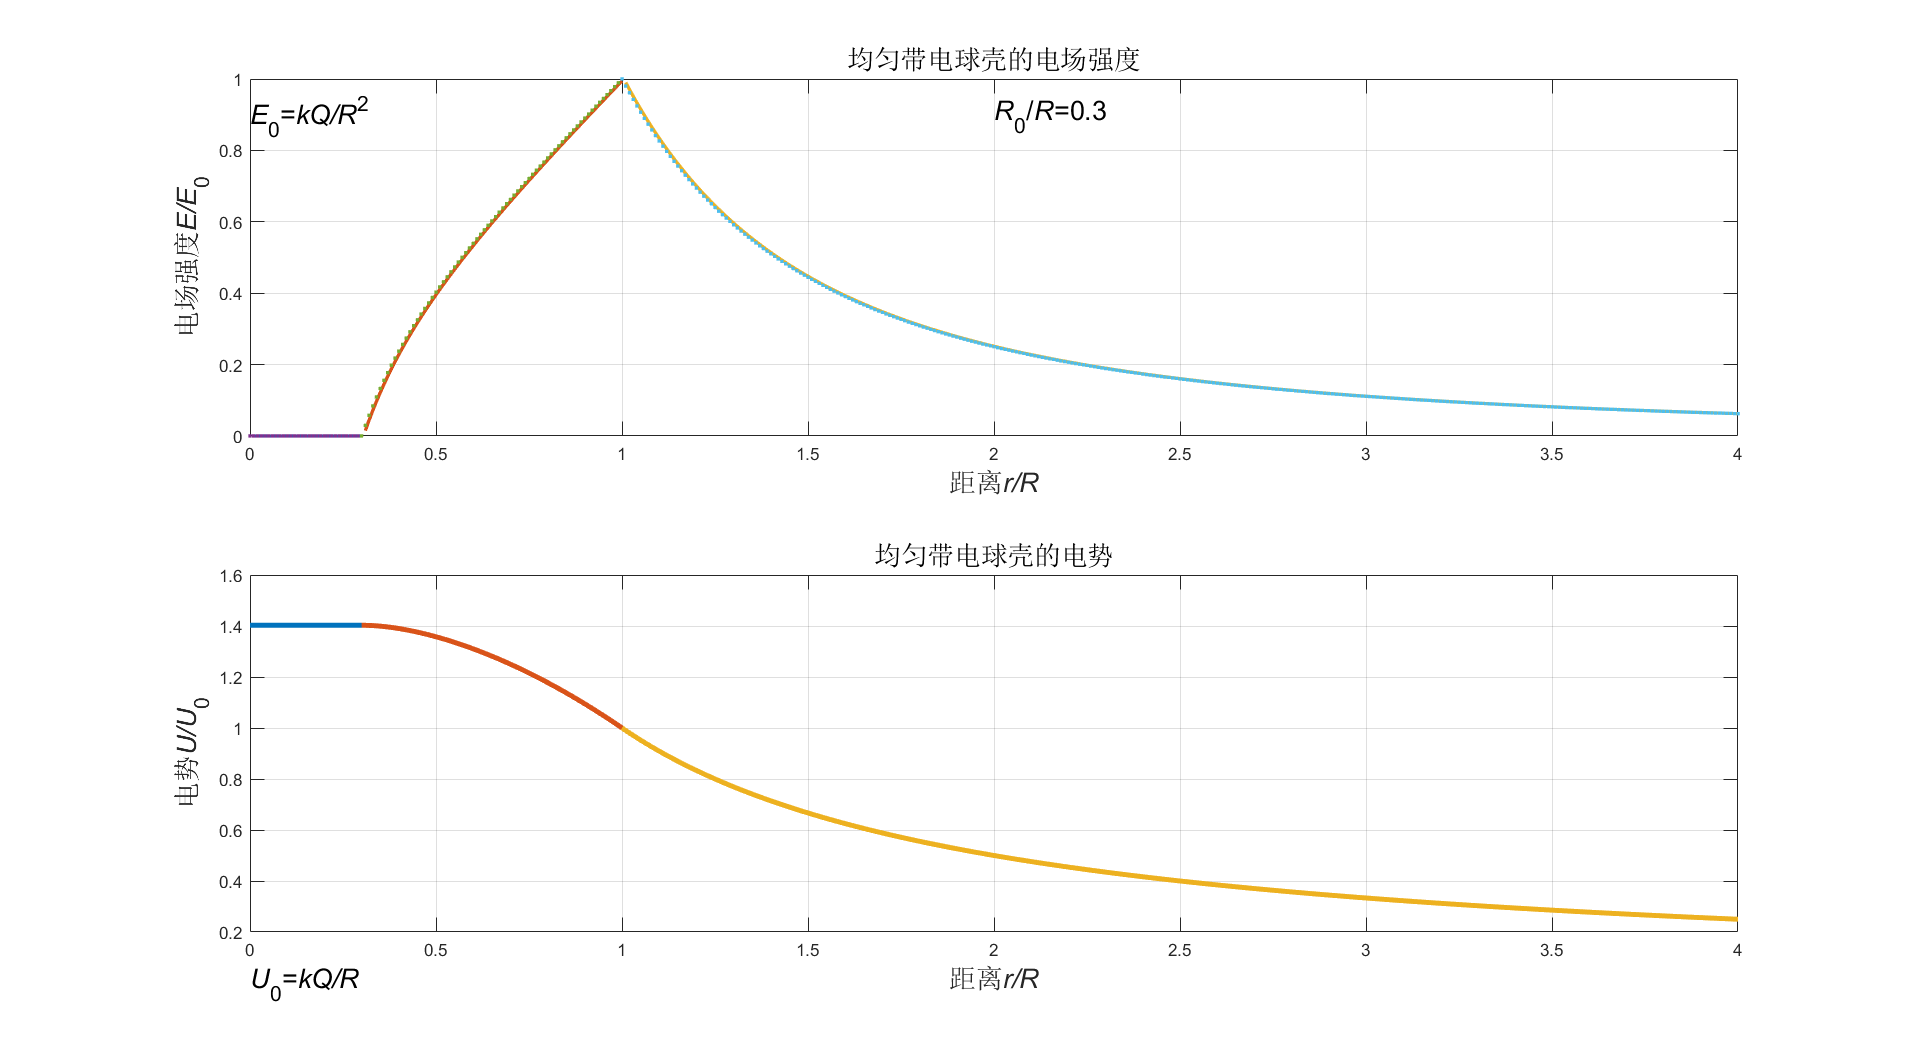
\includegraphics[scale=0.15]{0.3.png}
		\caption{内半径与外半径之比为0.3时均匀带点球壳电场强度和电势}
	\end{figure}
	\begin{figure}[H]
		\centering
		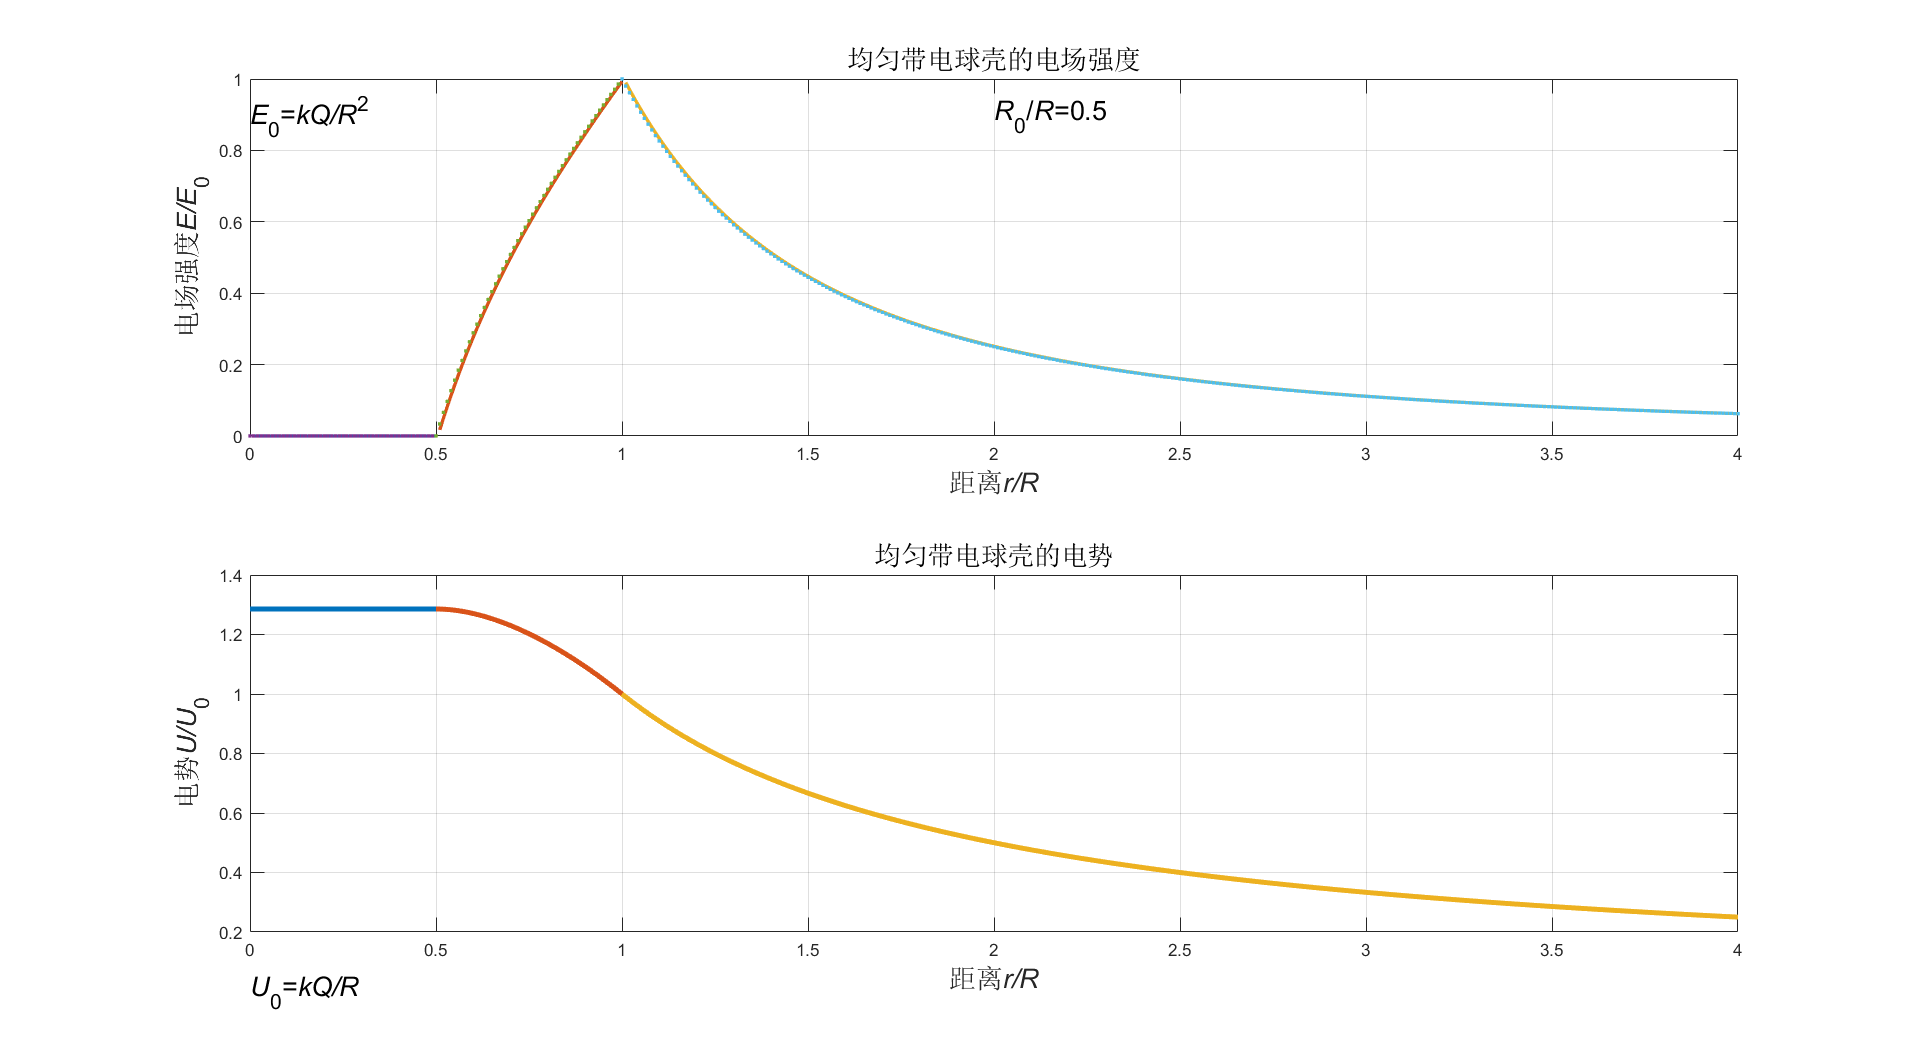
\includegraphics[scale=0.15]{0.5.png}
		\caption{内半径与外半径之比为0.5时均匀带点球壳电场强度和电势}
	\end{figure}
	\begin{figure}[H]
		\centering
		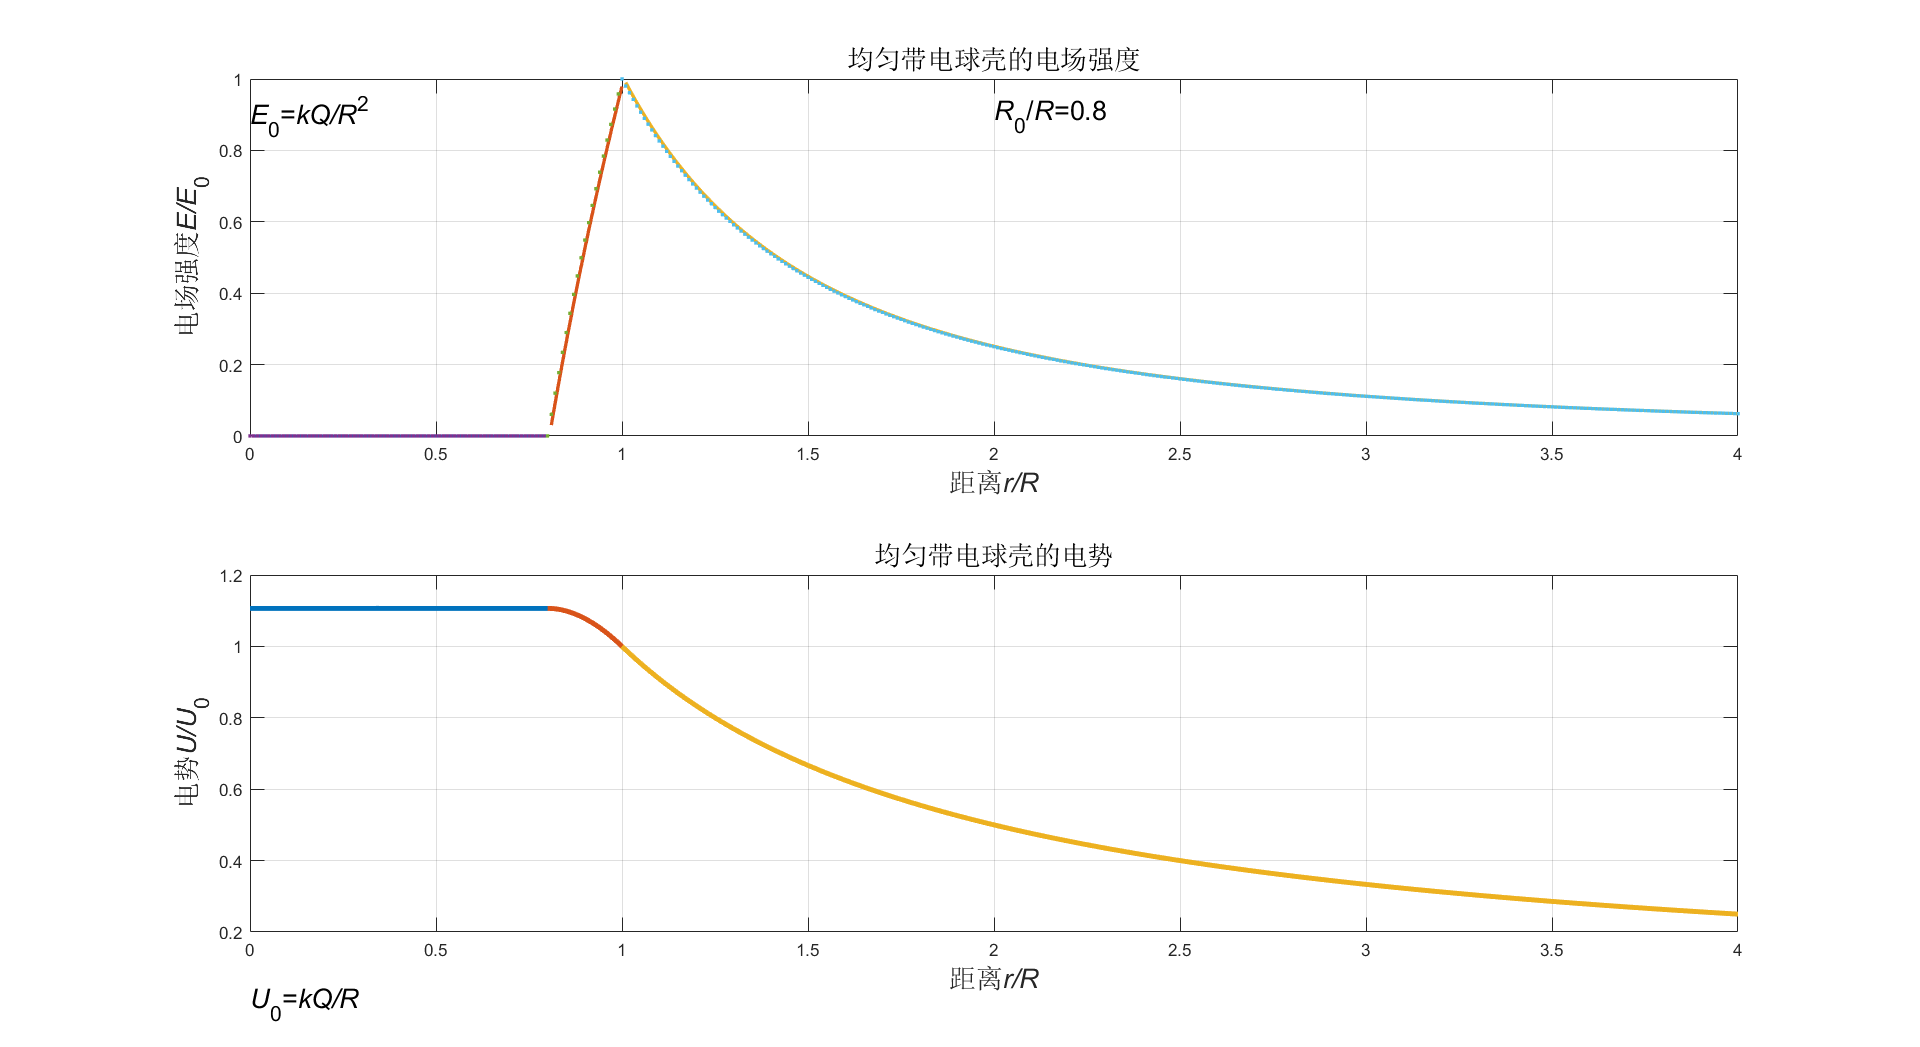
\includegraphics[scale=0.15]{0.8.png}
		\caption{内半径与外半径之比为0.8时均匀带点球壳电场强度和电势}
	\end{figure}
	\begin{figure}[H]
		\centering
		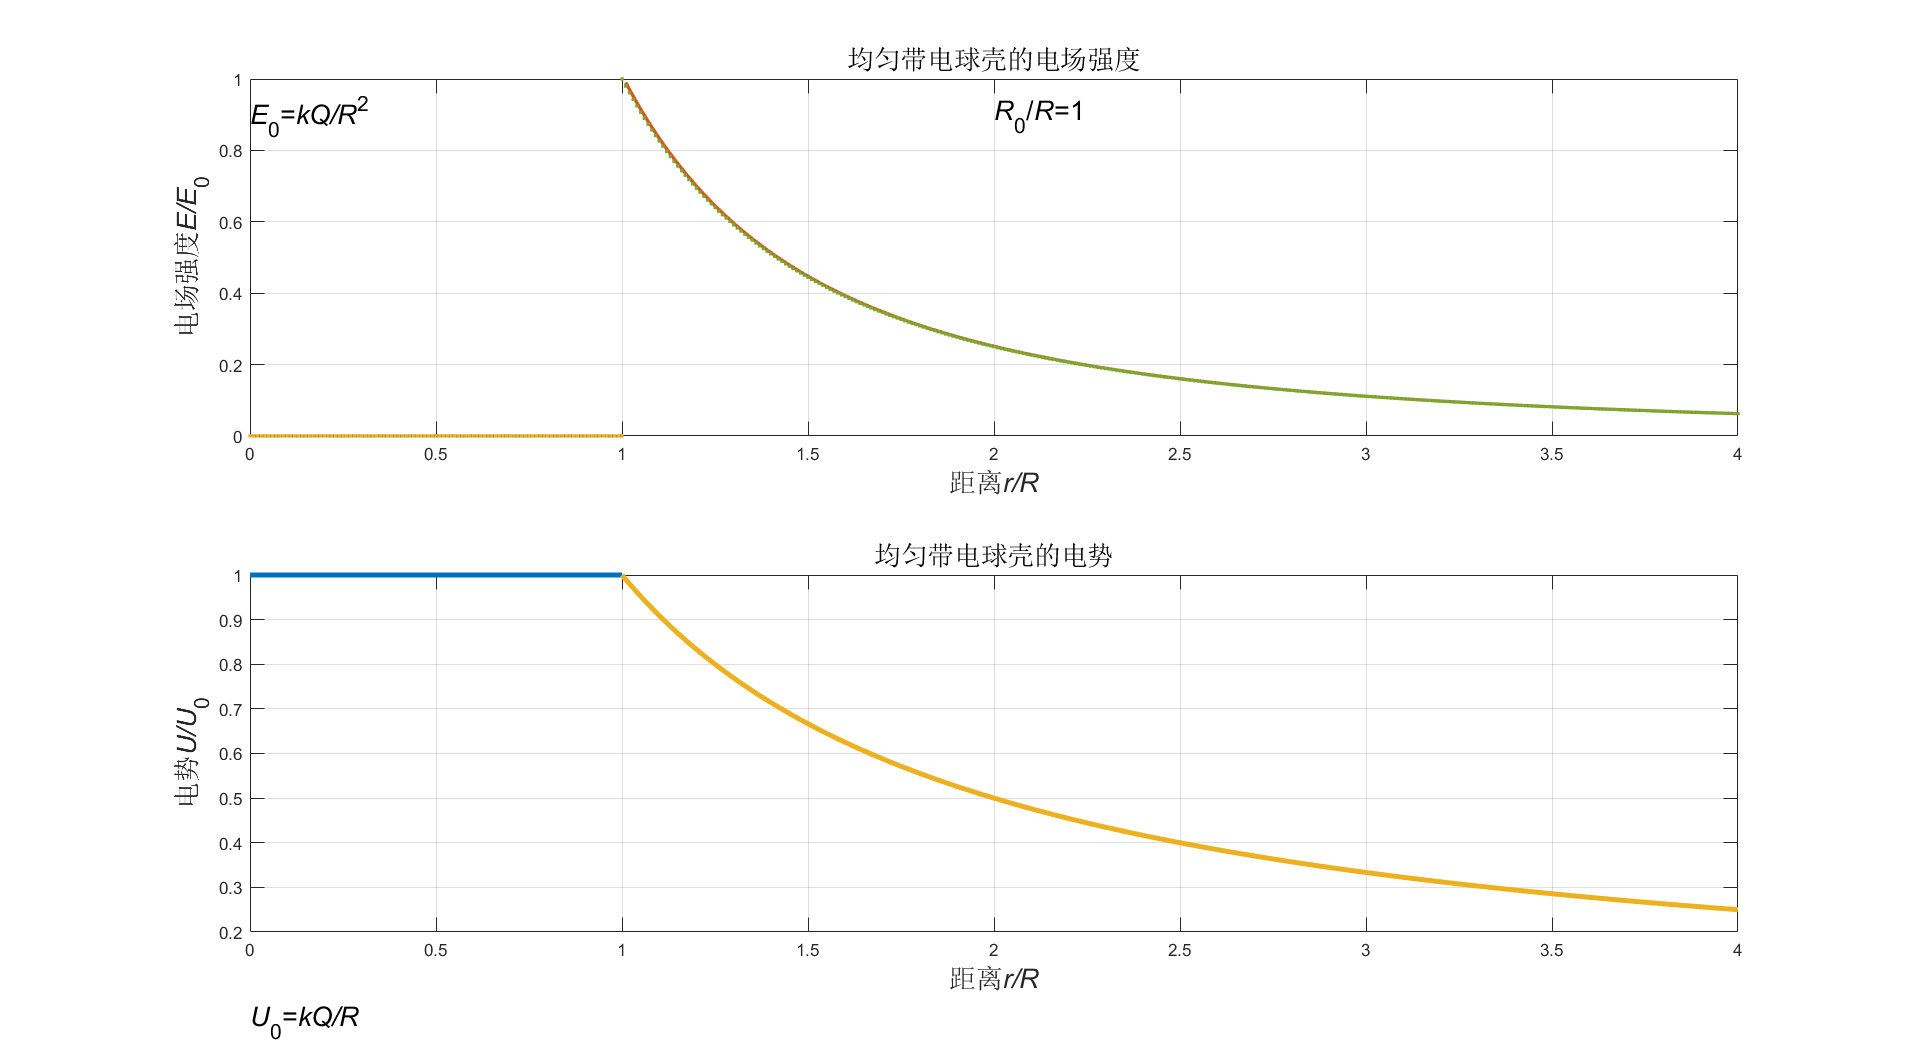
\includegraphics[scale=0.15]{1.png}
		\caption{内半径与外半径之比为1时均匀带点球壳电场强度和电势}
	\end{figure}
	\begin{figure}[H]
		\centering
		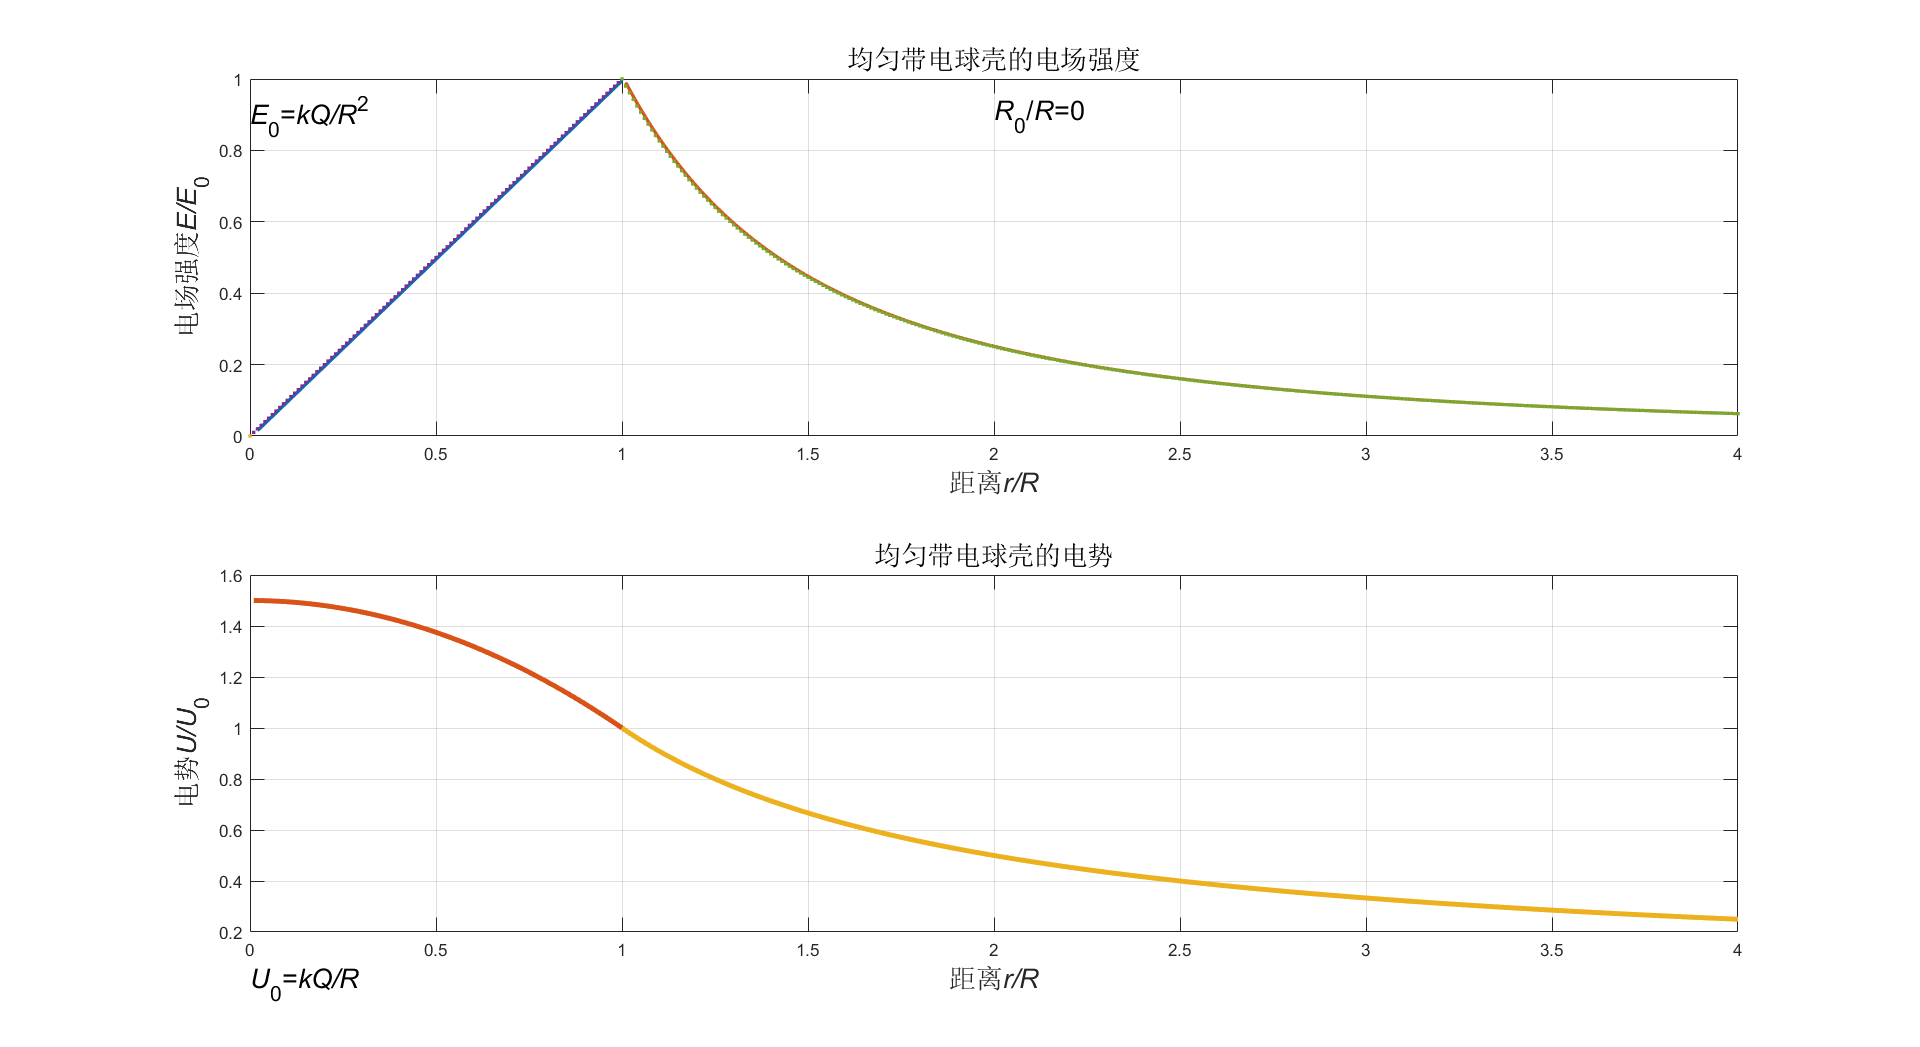
\includegraphics[scale=0.15]{0.png}
		\caption{内半径与外半径之比为0时均匀带点球壳电场强度和电势}
	\end{figure}
	\subsubsection{规律探究}
	\par 电场强度和电势随距离变化的规律
	\par 对于球壳内部空腔区域,电场强度始终为零,电势为常数。在球壳本身区域,电场强度随着距离增大而增大,电势则随着距离增大而减小。对于球壳外部区域,电场强度随着距离的增大而减小,遵循平方反比定律;电势也随着距离的增大而减小,遵循反比定律。
	\par 不同的球壳厚度会影响球壳内部区域的电场强度和电势。具体地,如果 $R_0$ 接近 $R$,即球壳厚度减小,球壳内部区域的电场强度会增大,而电势差会减小。如果球壳非常薄,$R_0$ 接近 $R$,那么球壳内部区域的电场强度会趋向于一个较大的恒定值,而电势则接近于在 $R$ 处的值。
	\subsection{运动电荷的磁场}
	\subsubsection{问题描述}
	\par 用Matlab仿真一带电量为q的电荷以速度v运动,求运动电荷产生磁感应强度。
	\subsubsection{公式推导}
	\par 对于一个带电量为 $q$,以速度 $\vec{v}$ 运动的点电荷,根据毕奥-萨伐尔定律:
	在极坐标系中,可得
	$$B=\frac{k_m qvsin\theta}{r^2}$$
	$\theta$是速度方向与场外矢径方向之间的夹角
	\subsubsection{代码解释}
	\par 代码主要实现两个功能。
	\par 第一部分是绘制直线电流的磁感应线。
	\par 首先通过输入比例系数k0来确定磁感应线的形状和大小。
	\par 然后根据给定的比例系数以及推导的公式,计算出每个点的半径r,并根据r生成对应的X、Y坐标。最后使用plot函数将磁感应线绘制出来,并添加图例、网格等元素。
	\begin{lstlisting}
    clear
    k0=input('请输入比例系数:');
    n=7;
    r=ones(1,n-1)*k0;
    r=[1,r];
    r=cumprod(r);
    theta=linspace(0,2*pi);
    X=cos(theta')*r;
    Y=sin(theta')*r;
	\end{lstlisting}
	\par 第二部分是绘制运动电荷产生的磁感应强度的分布面。
	\par 根据给定的参数rm生成半径r和角度th的向量。然后利用meshgrid函数生成对应的极坐标矩阵TH和R,并将其转化为笛卡尔坐标系下的X、Y坐标。
	\par 根据公式计算出对应的磁感应强度B。
	\par 最后使用surf函数将磁感应强度的分布面绘制出来,并添加图例、轴标签等元素。
	\begin{lstlisting}
    clear
    rm=2;
    r=0.2:0.1:rm;
    th=linspace(0,2*pi,50);
    [TH,R]=meshgrid(th,r);
    [X,Y]=pol2cart(TH,R);
    B=Y./R.^3;
	\end{lstlisting}
	\subsubsection{结果展示}
	\begin{figure}[H]
		\centering
		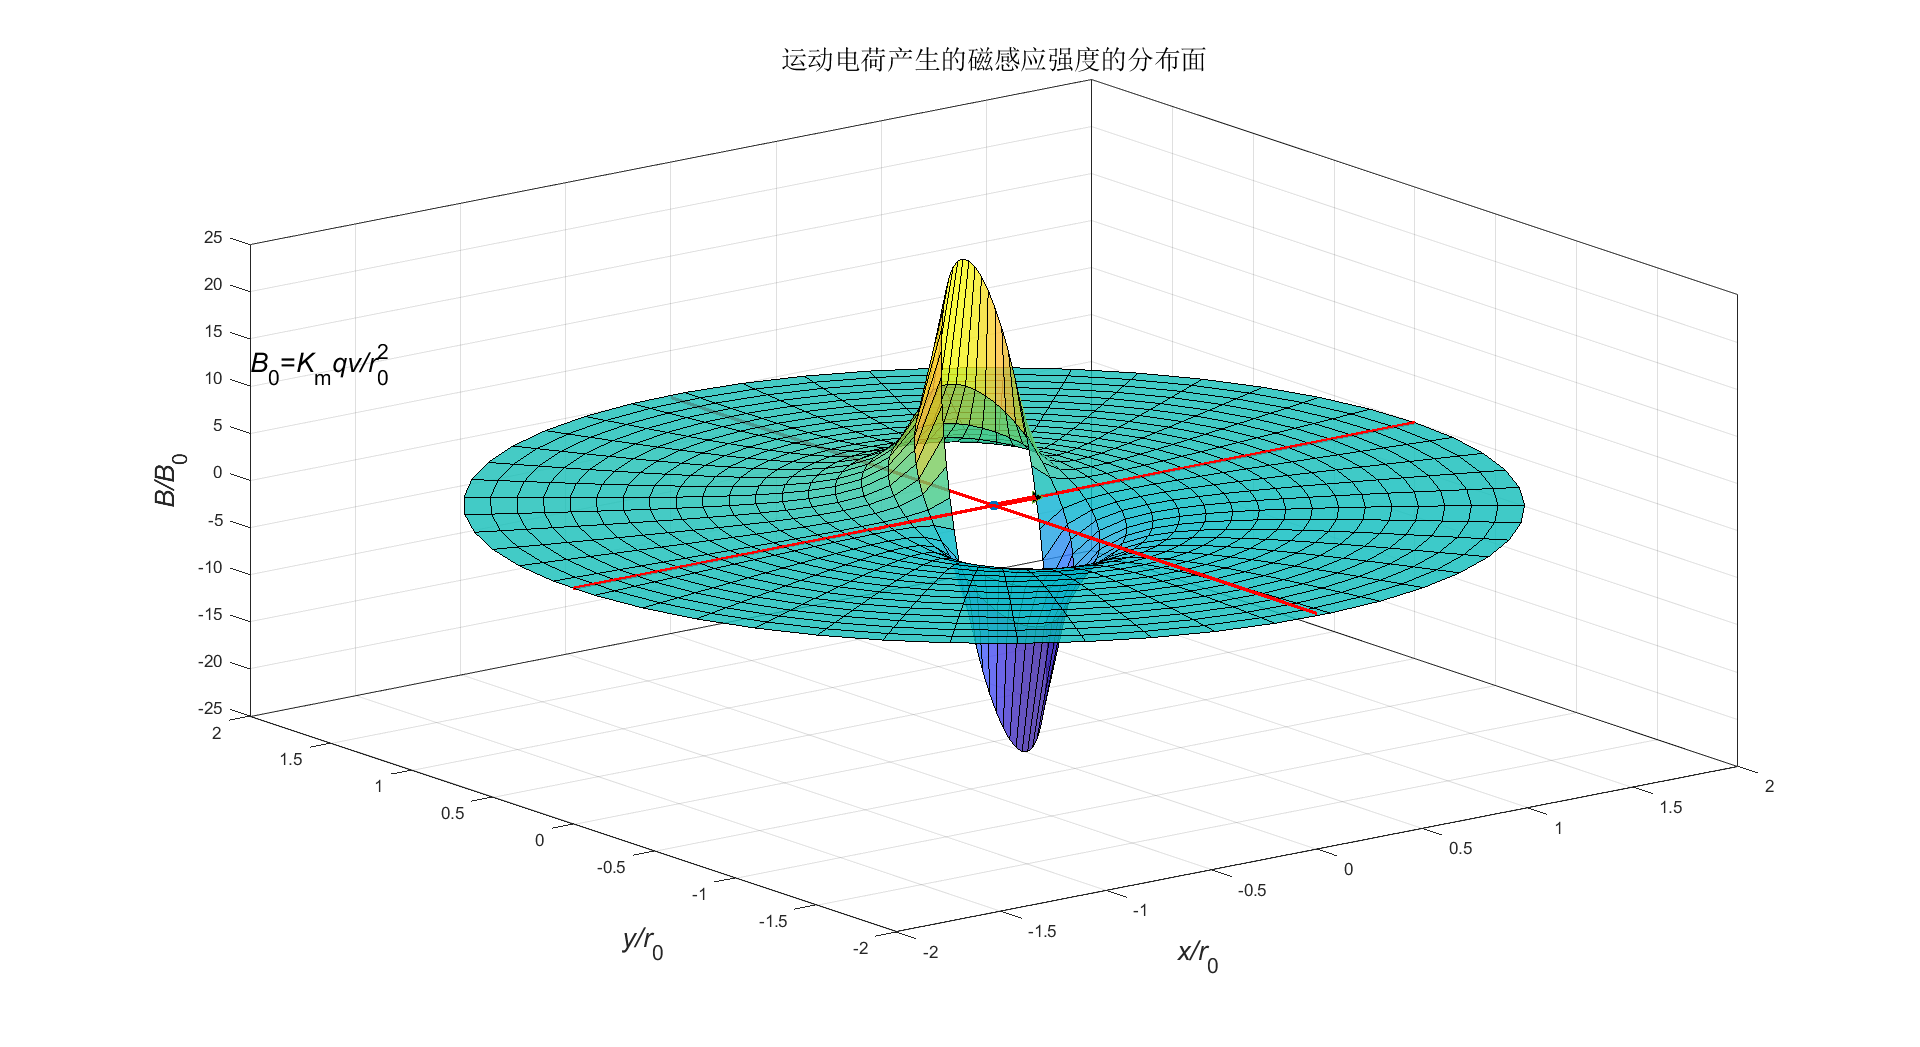
\includegraphics[scale=0.15]{5_1.2_1.png}
		\caption{运动电荷产生的磁感应强度的分布面}
	\end{figure}
	\begin{figure}[H]
		\centering
		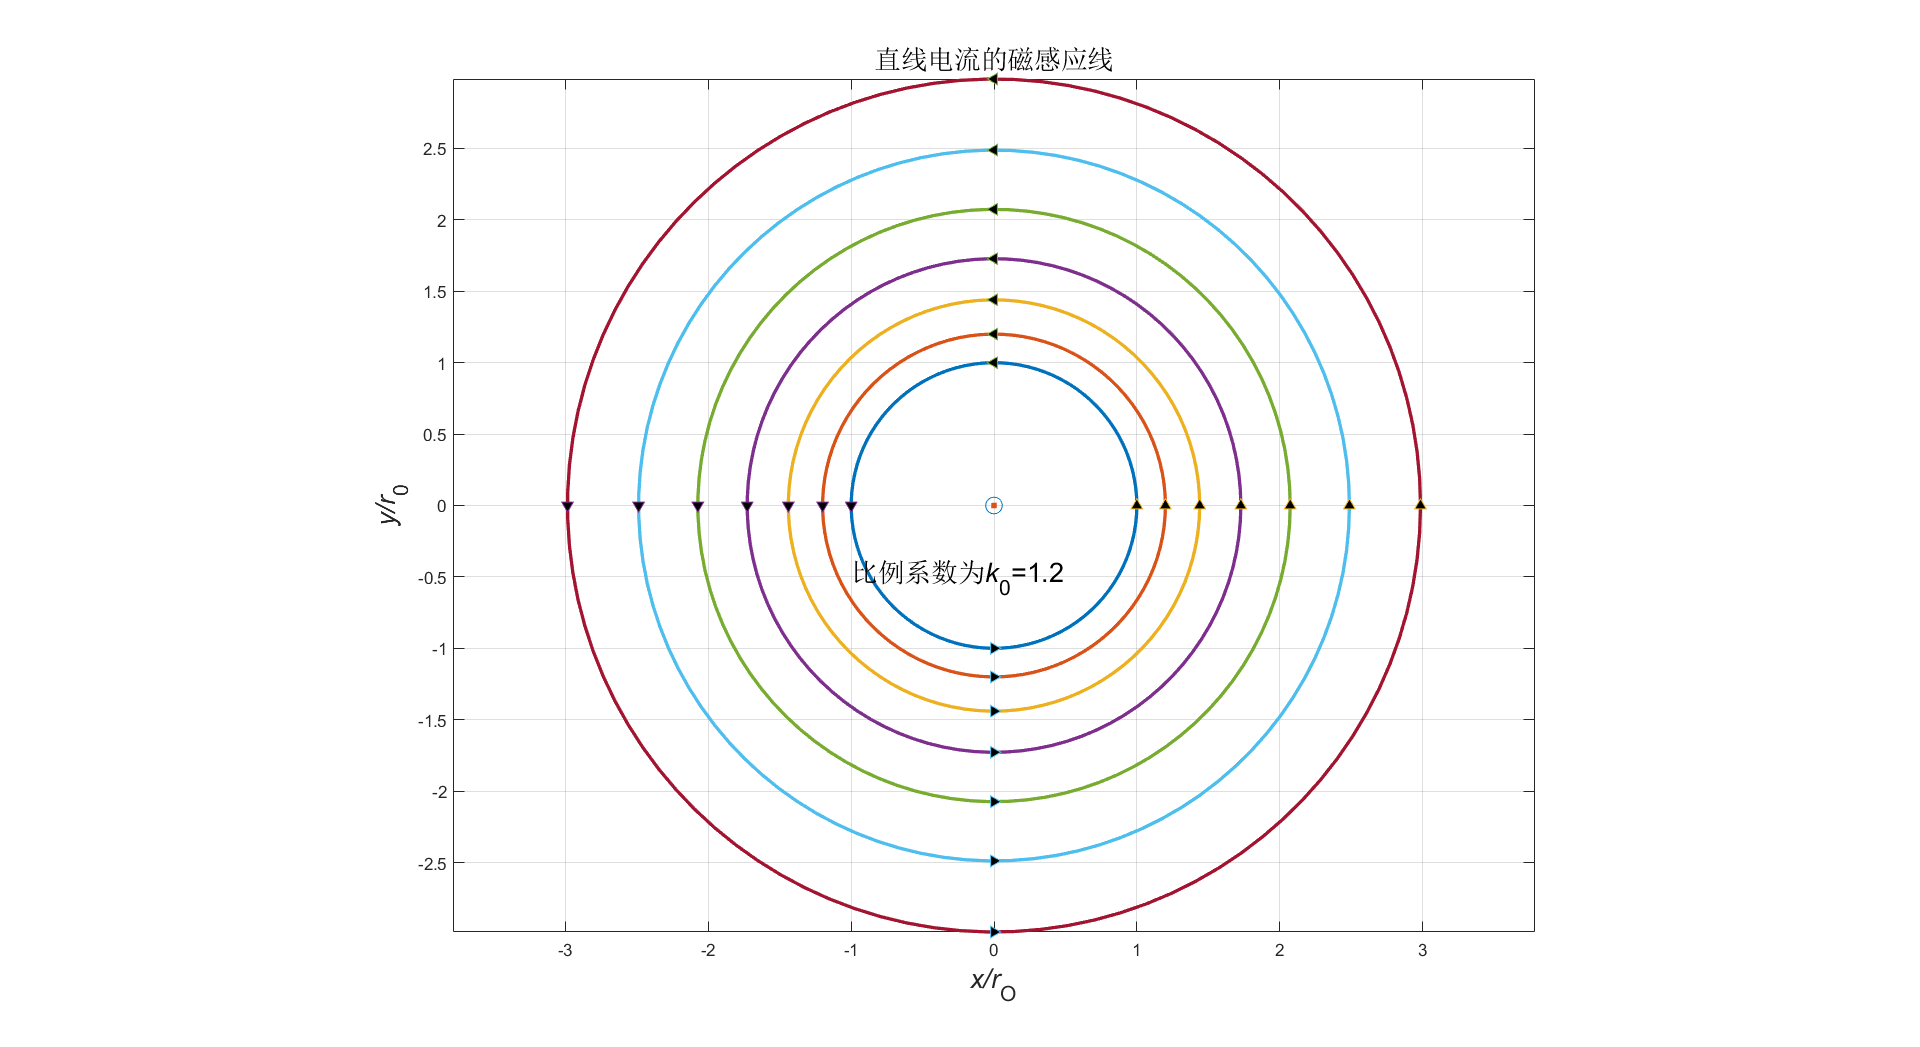
\includegraphics[scale=0.15]{5_1.2_2.png}
		\caption{比例系数为1.2时,直线电流的磁感应线}
	\end{figure}
	\begin{figure}[H]
		\centering
		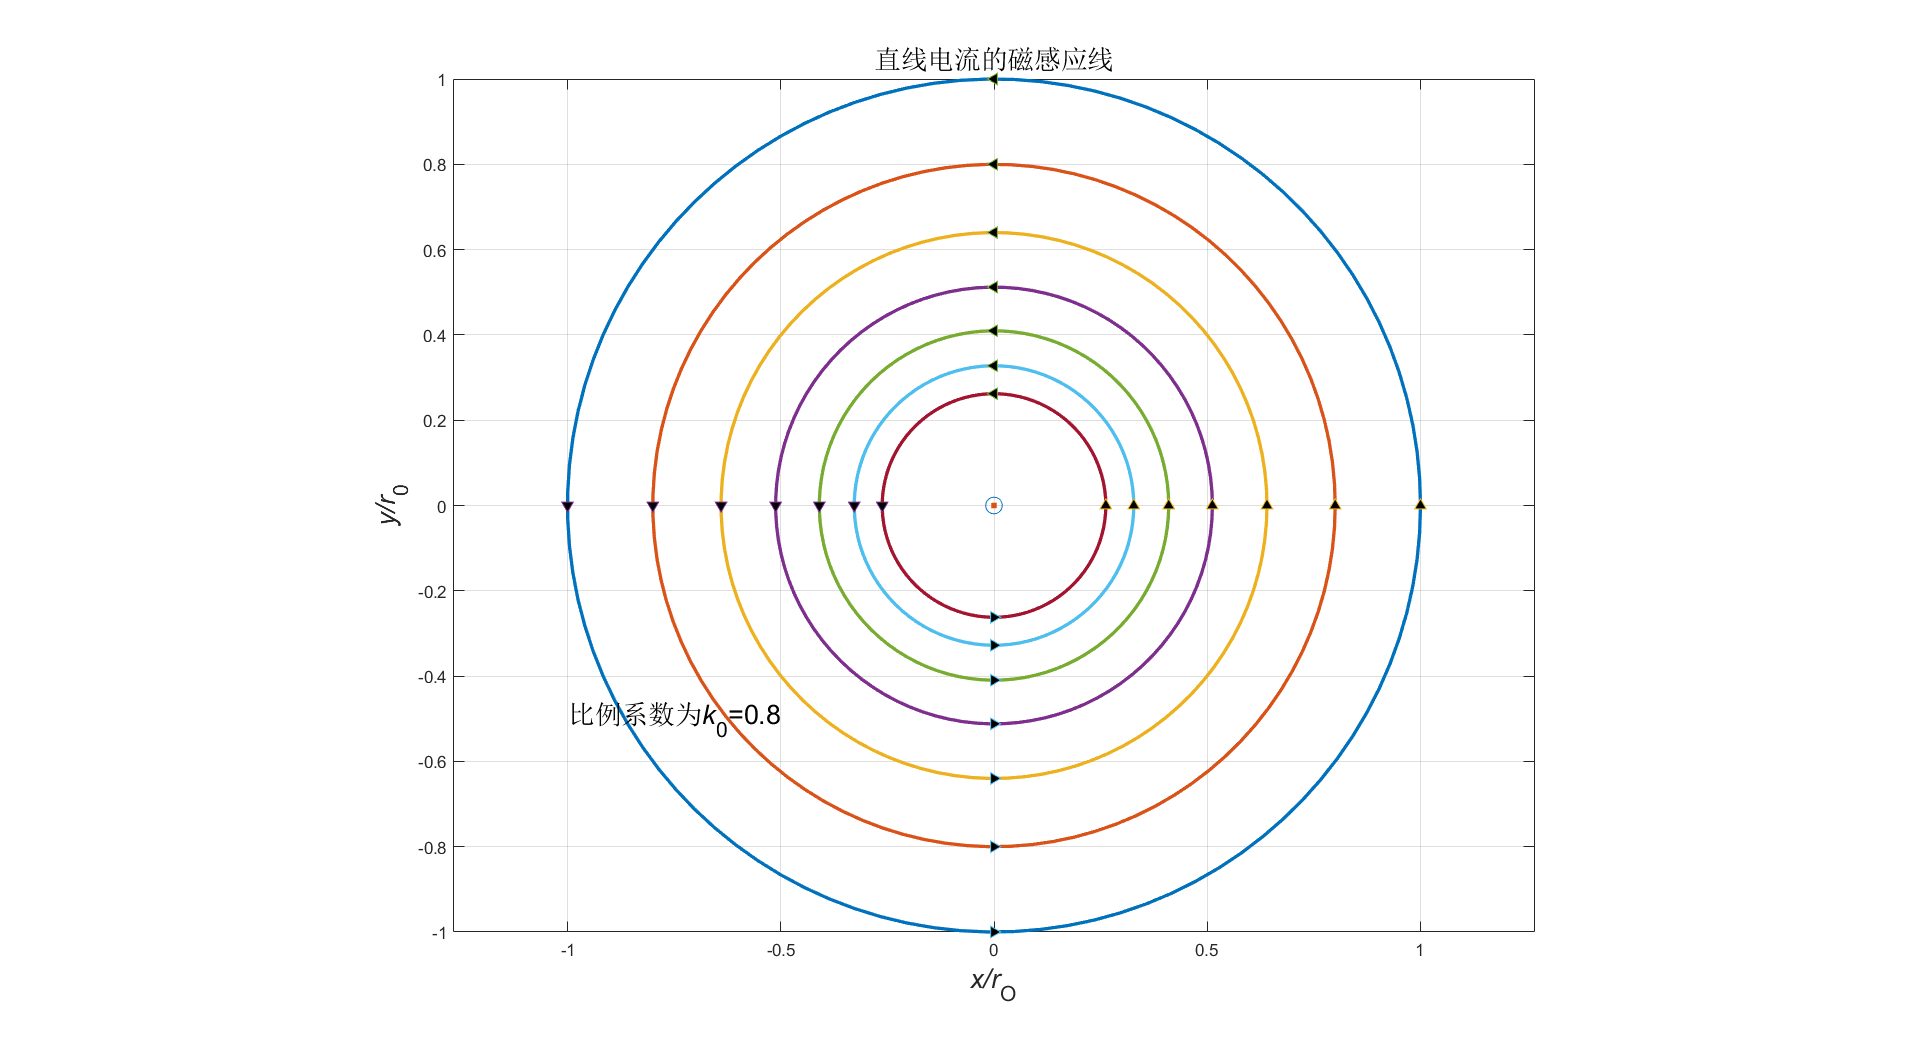
\includegraphics[scale=0.15]{5_0.8.png}
		\caption{比例系数为0.8时,直线电流的磁感应线}
	\end{figure}
	\subsubsection{规律探究}
	\par 运动电荷产生的磁感应强度分布规律
	\par 沿速度方向和反方向,磁感应强度均为0;在垂直于速度的方向,磁感应强度的大小与距离的平方成反比。
	\par 在其他方向,磁感应强度的大小仍与距离的平方成反比,但受到方向因子$sin\theta$的限制,在同样的距离内,其大小比速度中垂线上的场强大小要小。
	\subsection{无线长直导线磁感应线分布规律}
	\subsubsection{问题描述}
	\par 用Matlab仿真无线长直线电流的磁感应线的分布,计算无限长通电直线的磁感应强度是多少?磁感应线是如何分布的?
	\subsubsection{公式推导}
	\par 假设有一根无限长直线电流通过导线,电流强度为I。我们将观察点设在距离导线某一点的距离为r处。根据毕奥-萨伐尔定律,任意一点的磁感应强度B可以表示为:$B = \frac{\mu_0 I}{2\pi r}$
	\par 其中,$\mu_0$是真空中的磁导率,I是电流强度,r是观察点到导线的距离。
	\par 利用单位面积的磁感应线数正比于B的大小的关系,设N条磁感应线通过的面积为S,那么1条磁感应线占有的面积为$\Delta S$
	\par 取两条磁感应线,到通电直线的距离分别为$r_0$和$r_1$,宽度分别为$\Delta r_0$和$\Delta r_1$,高度为h,那么他们占有的面积分别为$h\Delta r_0$和$h\Delta r_1$。
	\par 根据
	$$B=\alpha \frac{N}{S}=\alpha \frac{1}{\Delta S}$$
	\par 并利用合比定理,可得
	$$r_1=\frac{1+\Delta r_0/2r_0}{1-\Delta r_0/2r_0} r_0=k_0 r_0$$
	$$\frac{\Delta r_0}{r_0}=\frac{\Delta r_1}{r_1}$$
	\par 同理可得:
	$$r_2=\frac{1+\Delta r_1/2r_1}{1-\Delta r_1/2r_1} r_1=k_1 r_1$$
	$$\frac{\Delta r_1}{r_1}=\frac{\Delta r_2}{r_2}$$
	而$k_1=k_0$所以无限长通电直导线的磁感应线与导线的距离形成等比数列。
	\subsubsection{代码解释}
	\par 首先对参数初始化并键入比例系数,用于确定磁感应线的半径。
	\par 然后初始化图形,定义磁感应线的数量为7条。
	\par 根据推导出的公式,计算出等比数列。
	\par 在窗口中绘制图形,并添加文字标记、网格等。
	\begin{lstlisting}
    clear 
    k0=input('请输入比例系数:');
    n=7;
    r=ones(1,n-1)*k0;%半径向量的初值
    r=[1,r];%补充第一个半径
    r=cumprod(r);%累积连乘形成半径向量
    theta=linspace(0,2*pi);%角度向量
    X=cos(theta')*r;%横坐标矩阵
    Y=sin(theta')*r;%纵坐标矩阵
	\end{lstlisting}
	\subsubsection{结果展示}
	\begin{figure}[H]
		\centering
		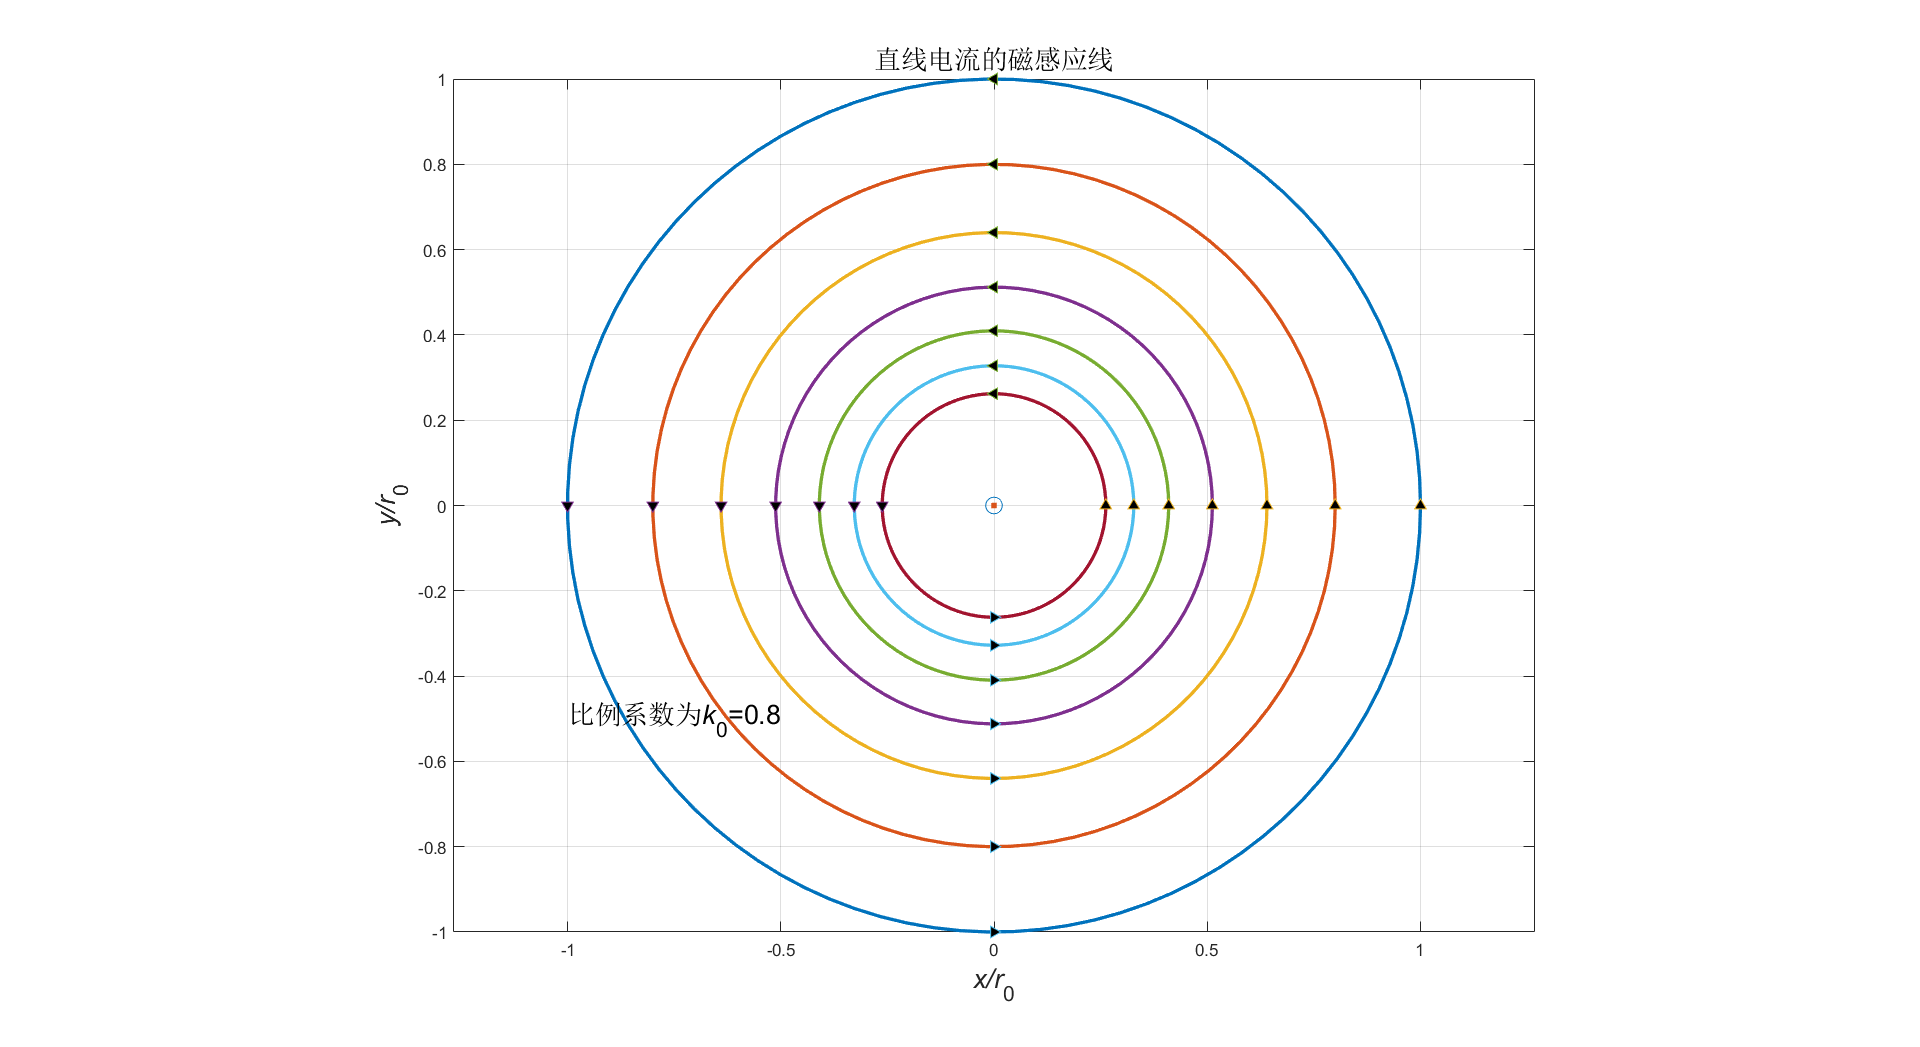
\includegraphics[scale=0.15]{6_0.8.png}
		\caption{比例系数为0.8时,无线长直导线磁感应线分布}
	\end{figure}
	\begin{figure}[H]
		\centering
		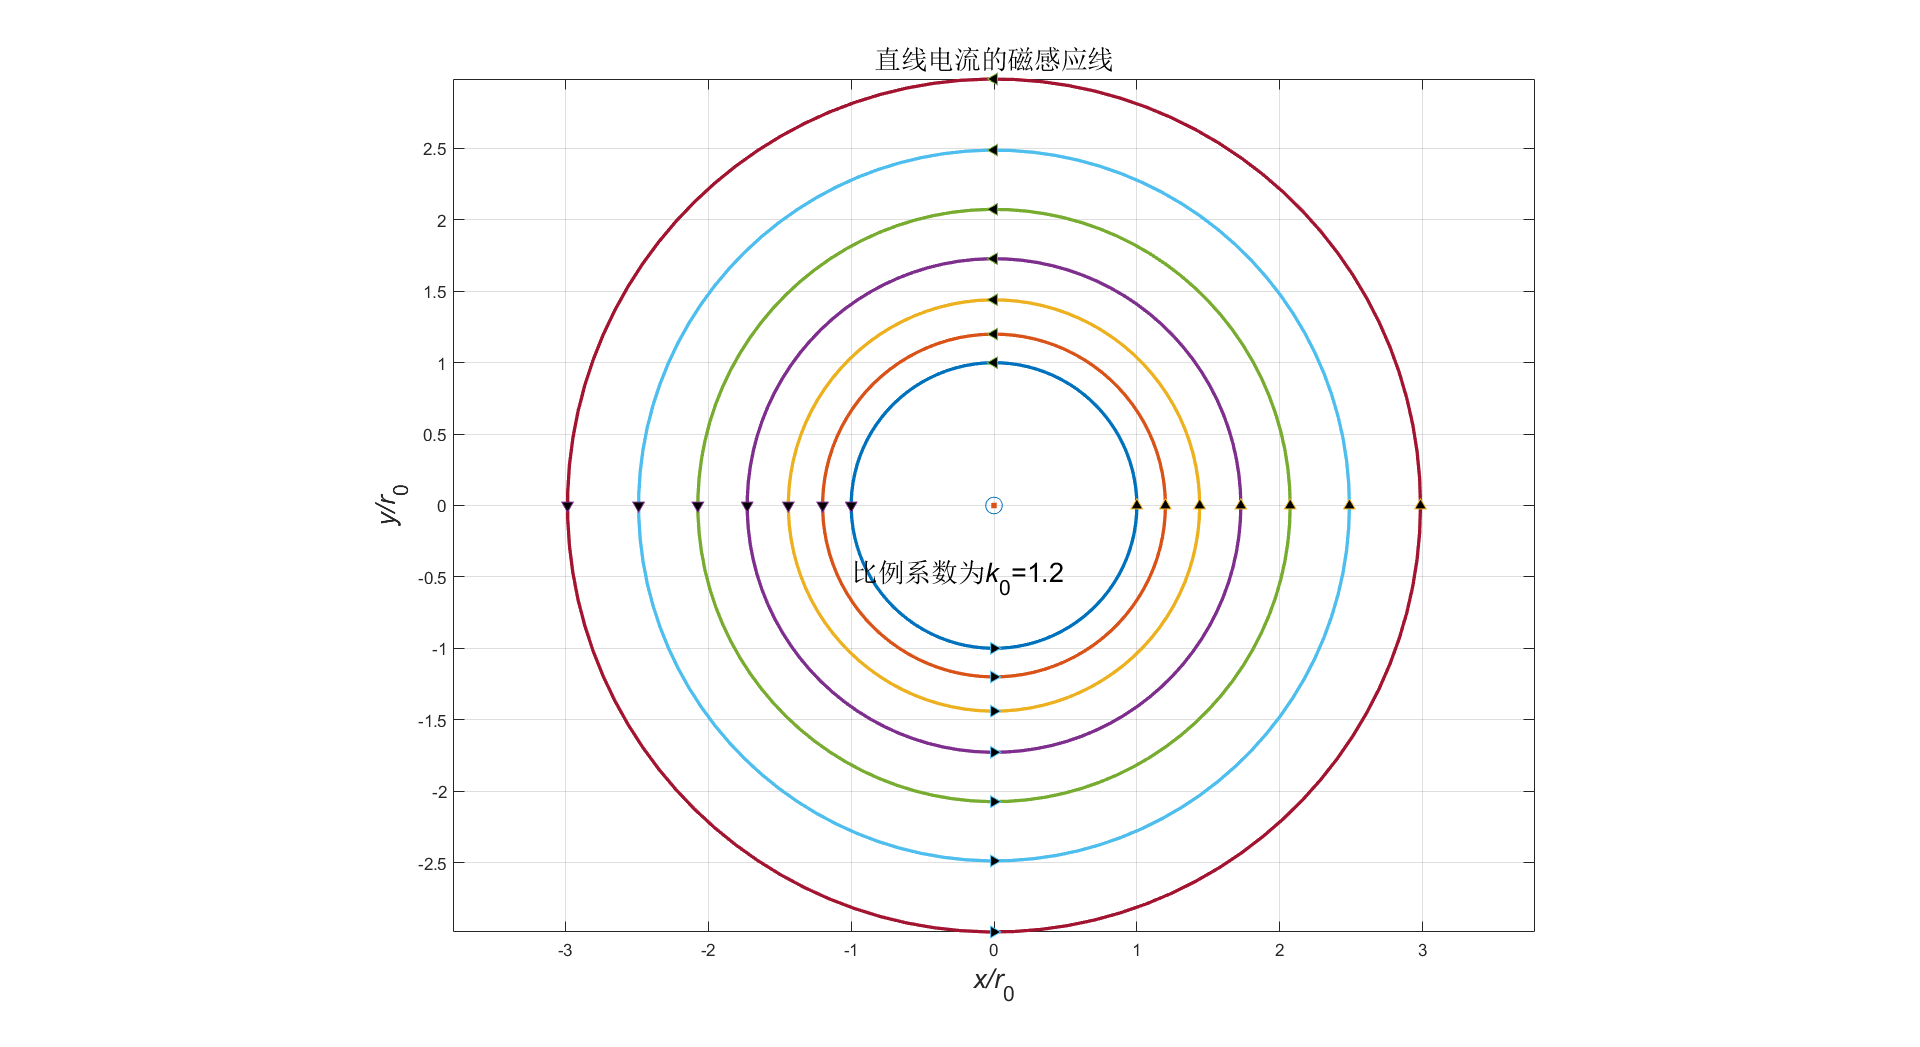
\includegraphics[scale=0.15]{6_1.2.png}
		\caption{比例系数为1.2时,无线长直导线磁感应线分布}
	\end{figure}	
	\section{复杂问题应用——静电场模拟系统}
	\subsection{方法论述}
	\par 在可视化模型呈现模块已经实现了单个点电荷二维平面内的电场强度和电势分布。本模块将基于前面已实现的的Matlab程序,计算并绘制多个电荷存在的二维平面的电场线分布及三维平面的电场线分布。
	已经推导过
	$$U = \frac{kQ}{r}$$
	$$E = -\nabla U$$
	所以可以现在matlab中求出各点的电势,用matlab自带的函数库求出电场强度并画出电力线在三维空间中的分布图。
	\subsection{Matlab程序及设计思路}
	\par 本部分仍只展示核心代码。
	\subsubsection{二维平面}
	\par 1. 清除已运行产生的同名变量,清楚干扰。加入电荷位置,电荷电性的输入口,以此来实现任意性。同时,加入了可以设置电场线间隔以及等势面间隔的输入口,使程序可控性更强。
	\begin{remark} 注:本程序电场线间隔应该为1-180;等势面差值间隔由设定点电荷决定最大值。不能太大,一般设置0.5左右;过小则运行时间太长。
	\end{remark}
	\par 初始化后,需要确定给出图像的显示范围。根据源点与各场点距离,由点电荷个数确定相关部分的循环次数。距离的反比是电位函数,既可以求导确定梯度进而画出电场线,又可以求得各场点的电位。而后通过循环语句求出各场点的电位。
	\par 求出电位值后,通过contour画出等势线,由t确定分度值。保持图像,此后在此图像上绘制电场线。通过循环语句和判断语句画出原点,正电荷以+表示,负电荷以o表示。
	\begin{lstlisting}
    G=size(a);
    g=G(1,1);
    R={};
    for i=(1:g) 
    R{1,i}=sqrt((X - a(i,1)).^2 + (Y-a(i,2)).^2 );
    %确定显示框内各点到各个点电荷的距离
    end
    U=zeros(size(X));
    %初始化,初始电势全为0
    for i=(1:g)
    U=U+Q(1,i)*(1./R{1,i});
    %将不同位置之于各极点的电势相加
    end
	\end{lstlisting}
	\par 电位处理完成后,需要处理电场强度。利用matlab自带的gradient函数求得两个维度方向的梯度,确定要引出电场线的角度间隔。由于电场线出自正电荷,终结至负电荷,所以从电荷画电场线。利用系统的streamline函数、循环语句和判断语句绘制正电荷和负电荷的电场线。
	\begin{lstlisting}
    [Ex,Ey]=gradient(-U,x(2)-x(1),y(2)-y(1));
    r0=0.1; %电场线起点半径
    b=(a1:a1:360-a1)*pi/180;
    for i=(1:g) 
    if Q(1,i)>0
    factor=1;
    else
    factor=-1
    end
    %任一个点电荷电场线的起点横坐标
    x1{1,i}=r0*cos(b)+a(i,1);
    %任一个点电荷电场线的起点纵坐标
    y1{1,i}=r0*sin(b)+a(i,2);
    %画任一个点电荷电场线
    streamline(X,Y,factor*Ex,factor*Ey,x1{1,i},y1{1,i});
    hold on;
    end
	\end{lstlisting}
	\par 最后补全图像的信息。
	\subsubsection{三维平面}
	\par 有了二维平面的基础,三维平面的实现更加容易。
	\par 首先,在二维程序的基础上,修改输入提醒为三维空间坐标,删去等势线差值输入。同时,需要增加z维度。
	\begin{lstlisting}
    G=size(a);
    g=G(1,1); %确定要画的电荷的个数,方便后边画图
    R={};
    for i=(1:g) 
    R{1,i}=sqrt((X - a(i,1)).^2 + (Y-a(i,2)).^2 + (Z - a(i,3)).^2); %确定显示框内各点到各个点电荷的距离
    end
    U=zeros(size(X)); %初始化,初始电势全为0
    for i=(1:g)
    U=U+Q(1,i)*(1./R{1,i}); %
    end
	\end{lstlisting}
	\par 除增加z维度外,还需更改电场线的显示方式。绘制三维空间的电场线时,点电荷在三维空间中的理想模型应该是球,故而电场线发散应该沿着$\varphi$和$\theta$两个方向,故而加入$\theta$相关的分度值和尺分度空间个数进而得出空间电场线分布。
	\begin{lstlisting}
    t=(a1:a1:360-a1)*pi/180;
    %电荷电场线的始末是θ角度和步长
    L=max(size(t));
    for j=(1:L)
    for i=(1:g) 
    if Q(1,i)>0
    factor=1;
    else
    factor=-1;
    end
    x1{1,i}=r0*cos(b)*sin(t(1,j))+a(i,1);
    y1{1,i}=r0*sin(b)*sin(t(1,j))+a(i,2);
    z1{1,i}=r0*sin(b)*cos(t(1,j))+a(i,3);
    streamline(X,Y,Z,factor*Ex,factor*Ey,factor*Ez,x1{1,i},y1{1,i},z1{1,i});
    hold on;
    end
    end
	\end{lstlisting}
	\subsection{方法应用示例}
	\subsubsection{方法的有效性及优越性}
	\par 有效性:可得出二维三维空间内的电场线分布情况,可得出二维平面内的电势分布情况。
	\par 优越性:相比参考的两种,该程序能实现二维空间内点电荷位置数量以及电性的任意选取,还能设置电场线和等势面的稠密。而且给出了三位空间内的电场线分布情况,同样实现点电荷位置数量以及电性的任意选取以及电场线稠密的设置。
	\subsubsection{二维平面测试示例}
	\begin{figure}[H]
		\centering
		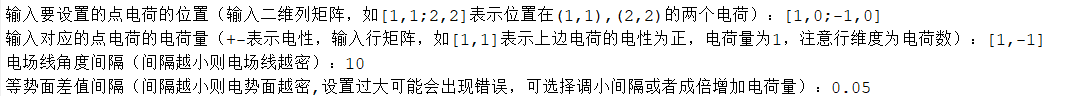
\includegraphics[scale=0.4]{ceshi1.png}
		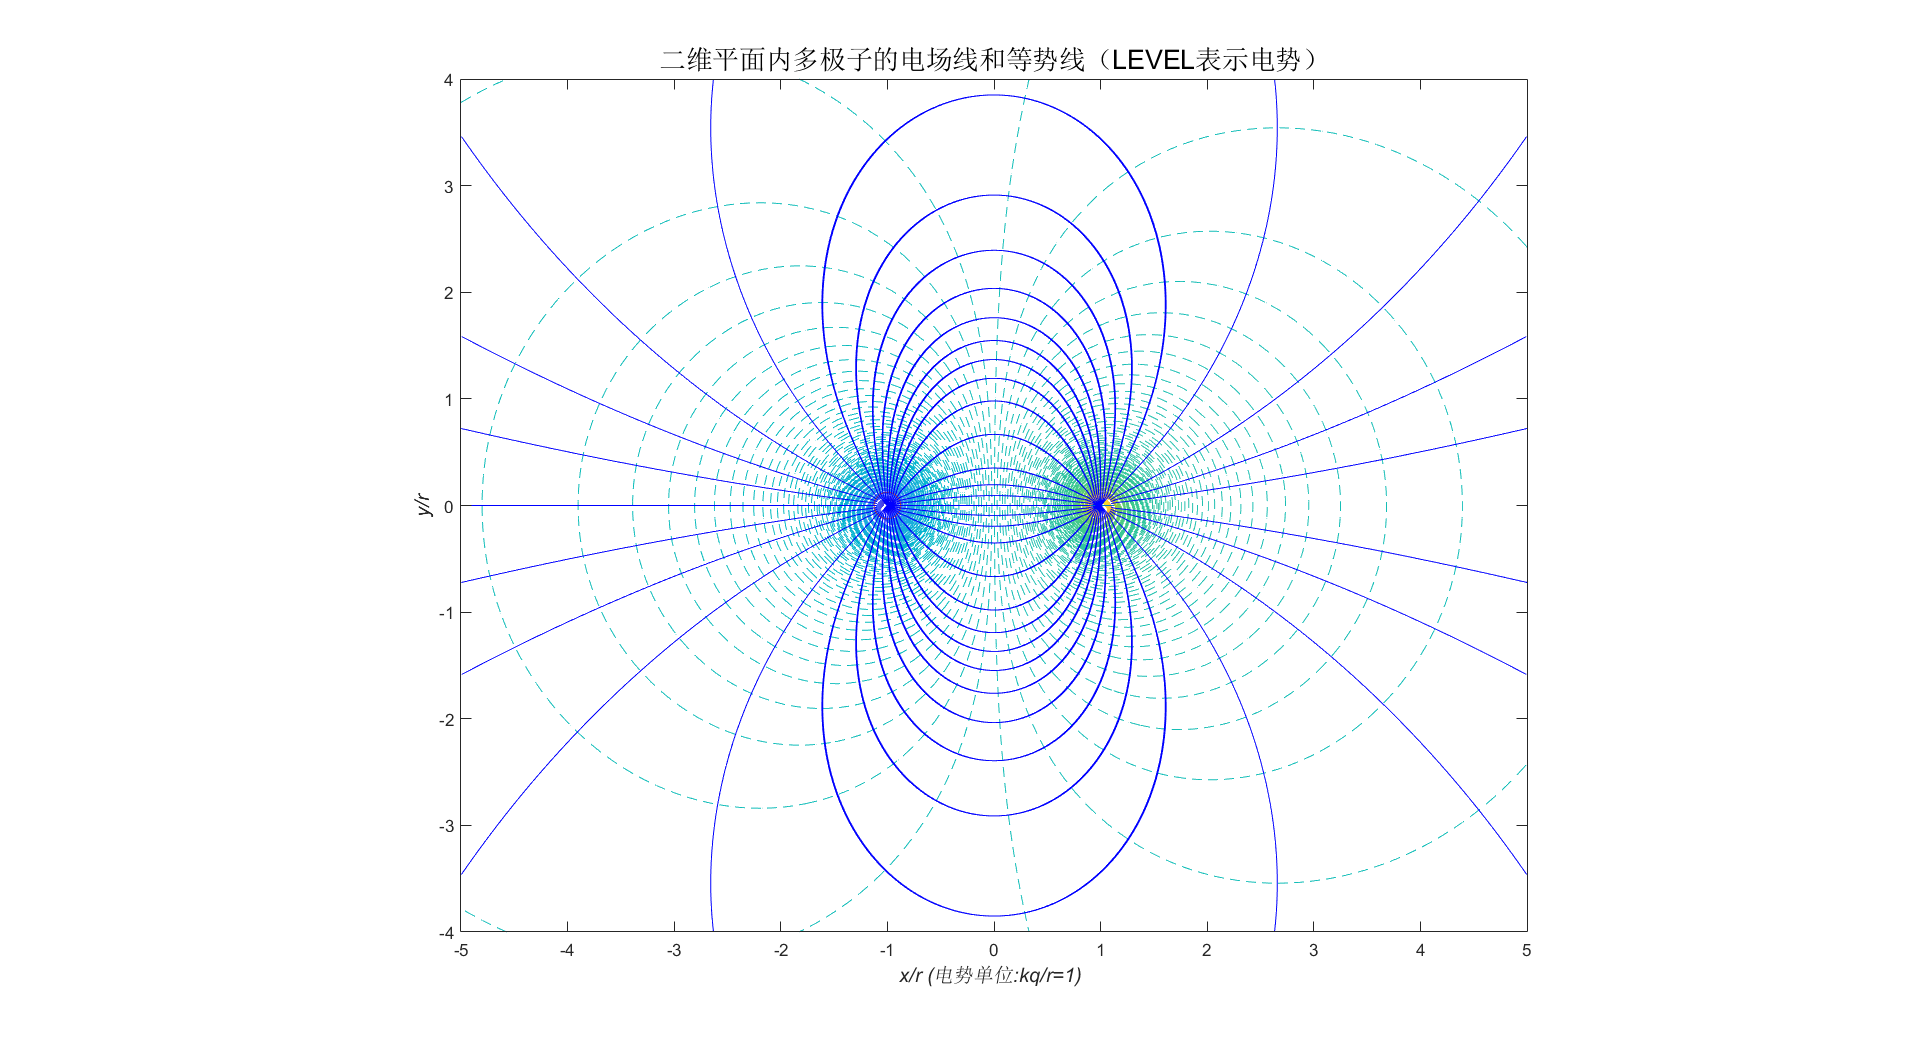
\includegraphics[scale=0.15]{测试1.png}
	\end{figure}
	\begin{figure}[H]
		\centering
		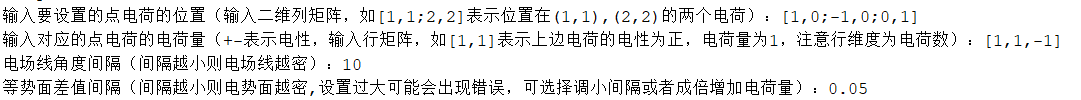
\includegraphics[scale=0.4]{ceshi2.png}
	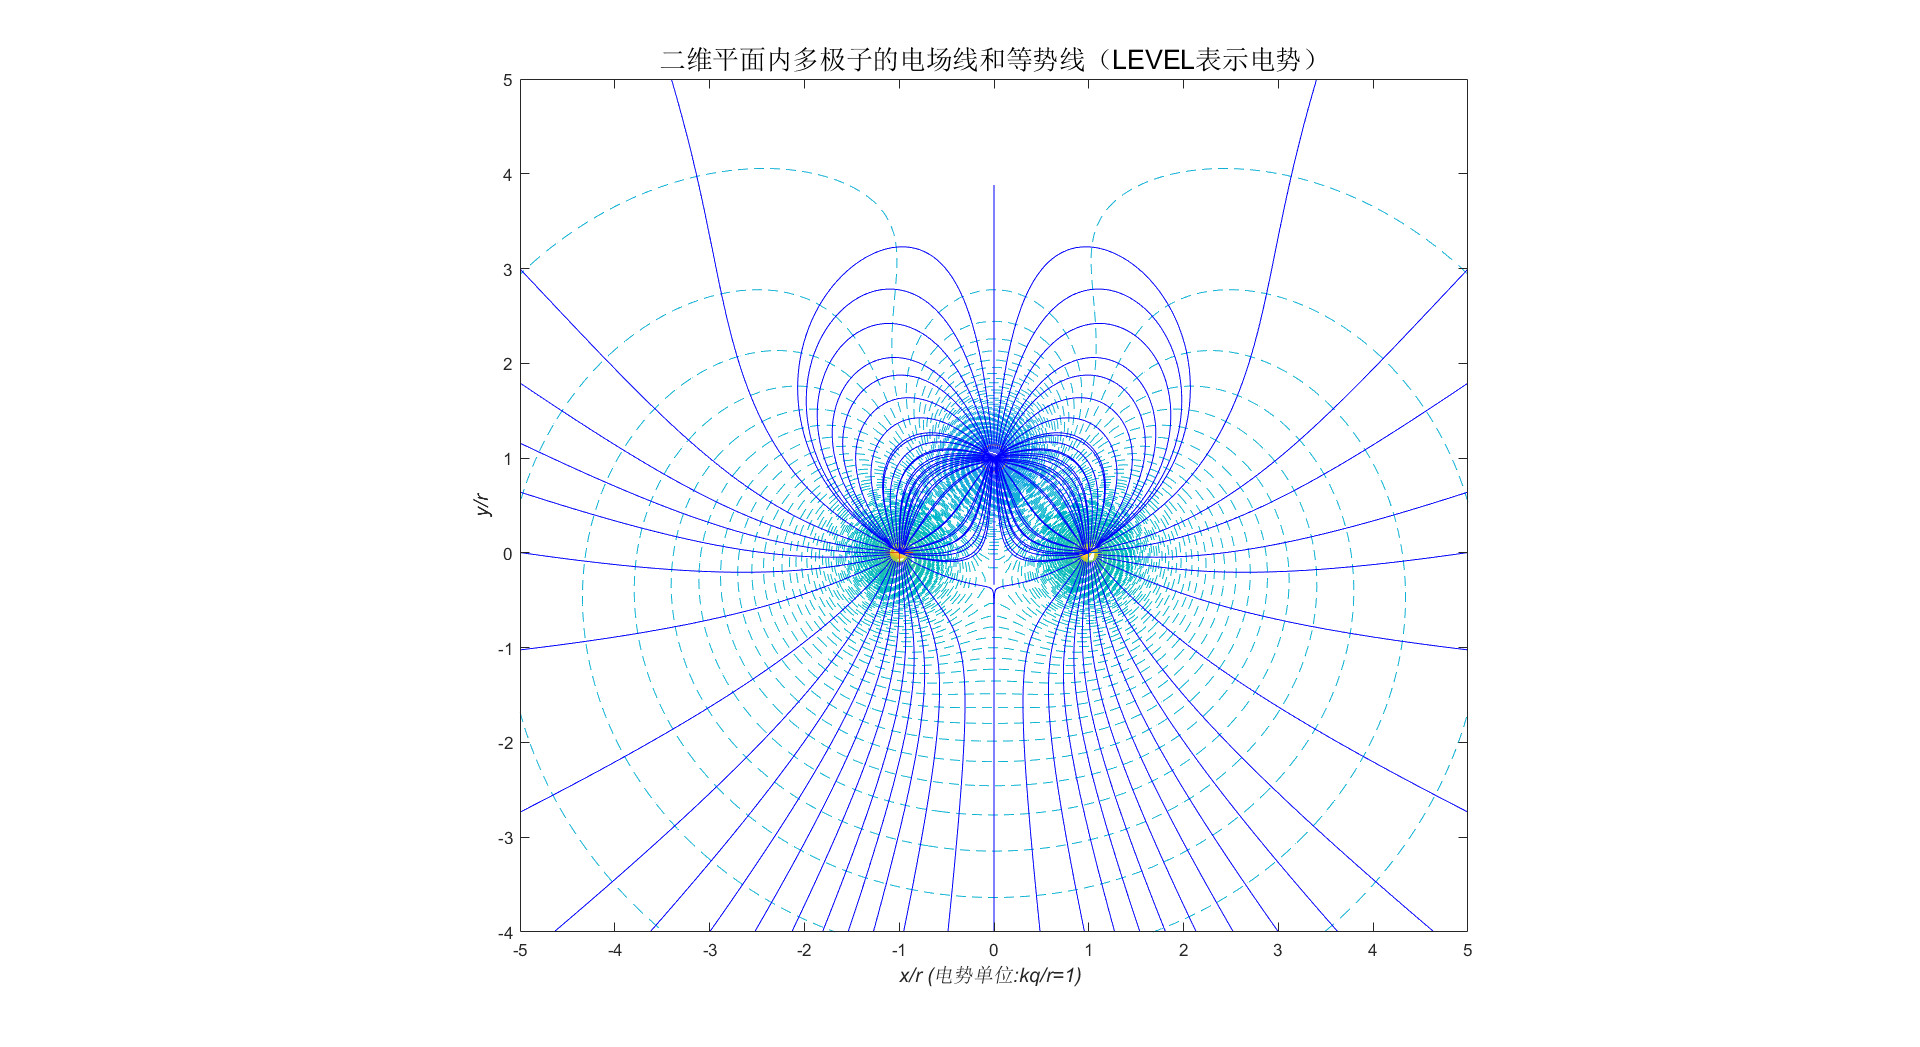
\includegraphics[scale=0.15]{测试2.png}
	\end{figure}
	\begin{figure}[H]
		\centering
		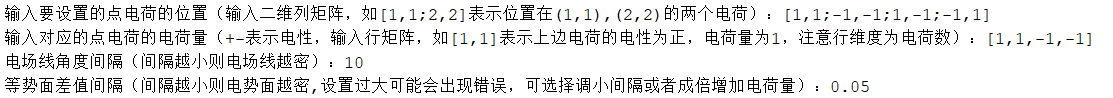
\includegraphics[scale=0.4]{ceshi3.png}
	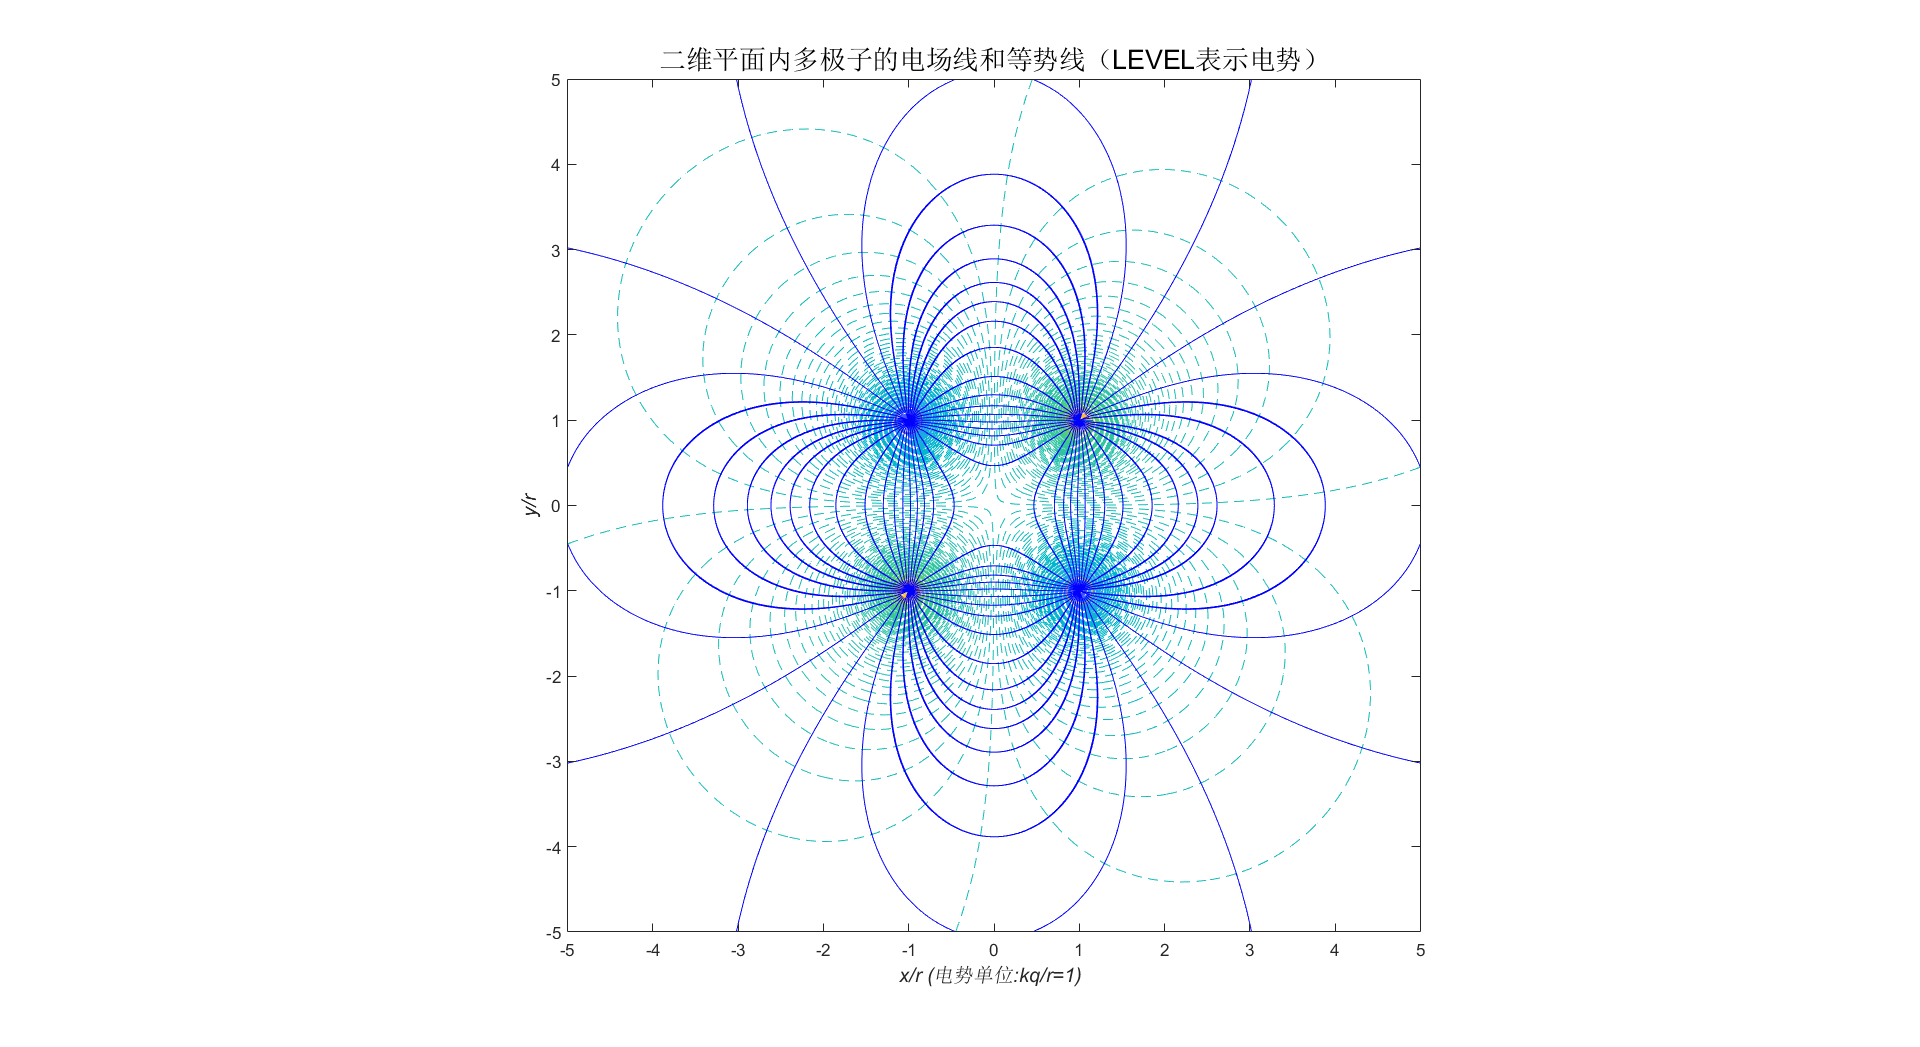
\includegraphics[scale=0.15]{测试3.png}
	\end{figure}
	\subsubsection{三维空间测试示例}
	\begin{figure}[H]
		\centering
		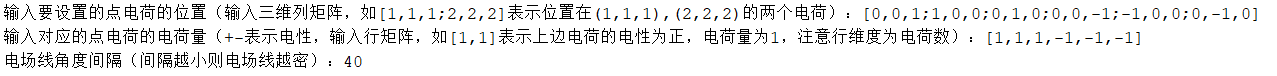
\includegraphics[scale=0.4]{ceshi4.png}
	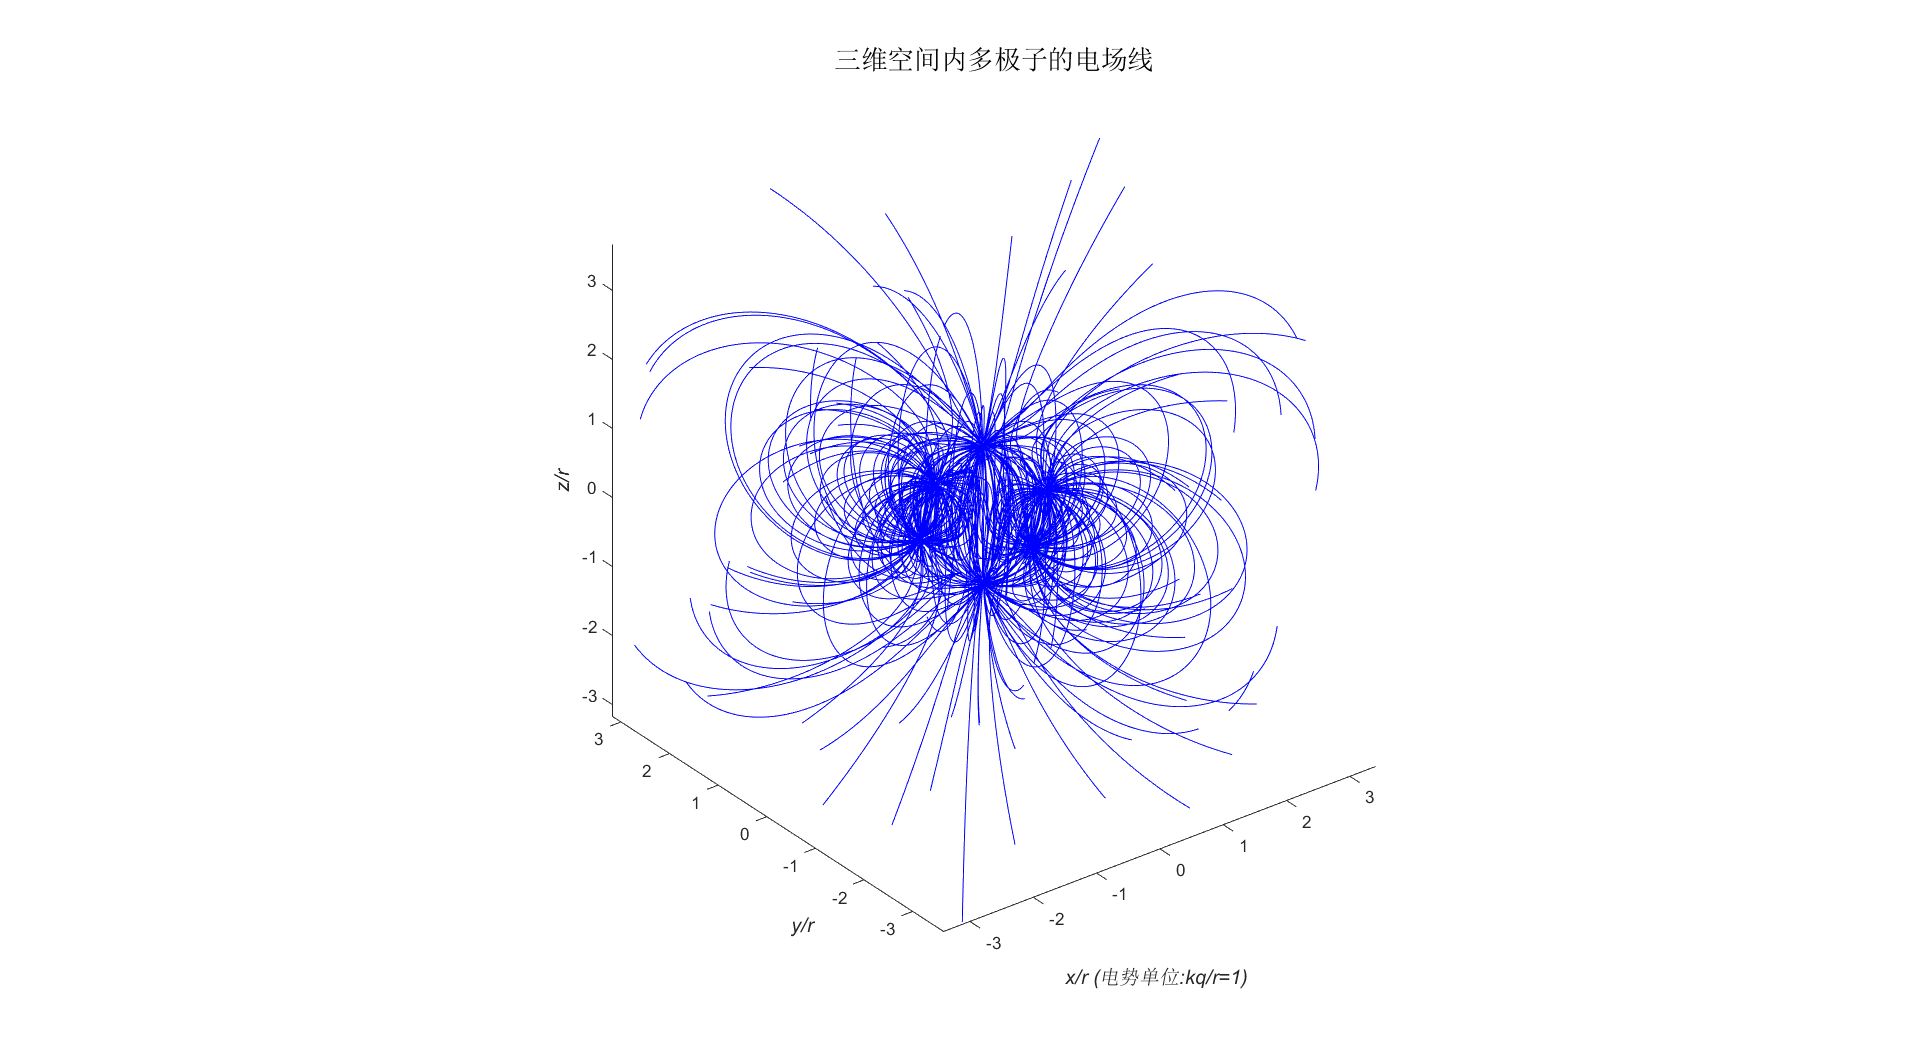
\includegraphics[scale=0.15]{测试4.png}
	\end{figure}
	\begin{figure}[H]
		\centering
		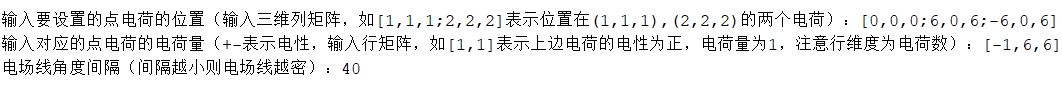
\includegraphics[scale=0.4]{ceshi5.png}
	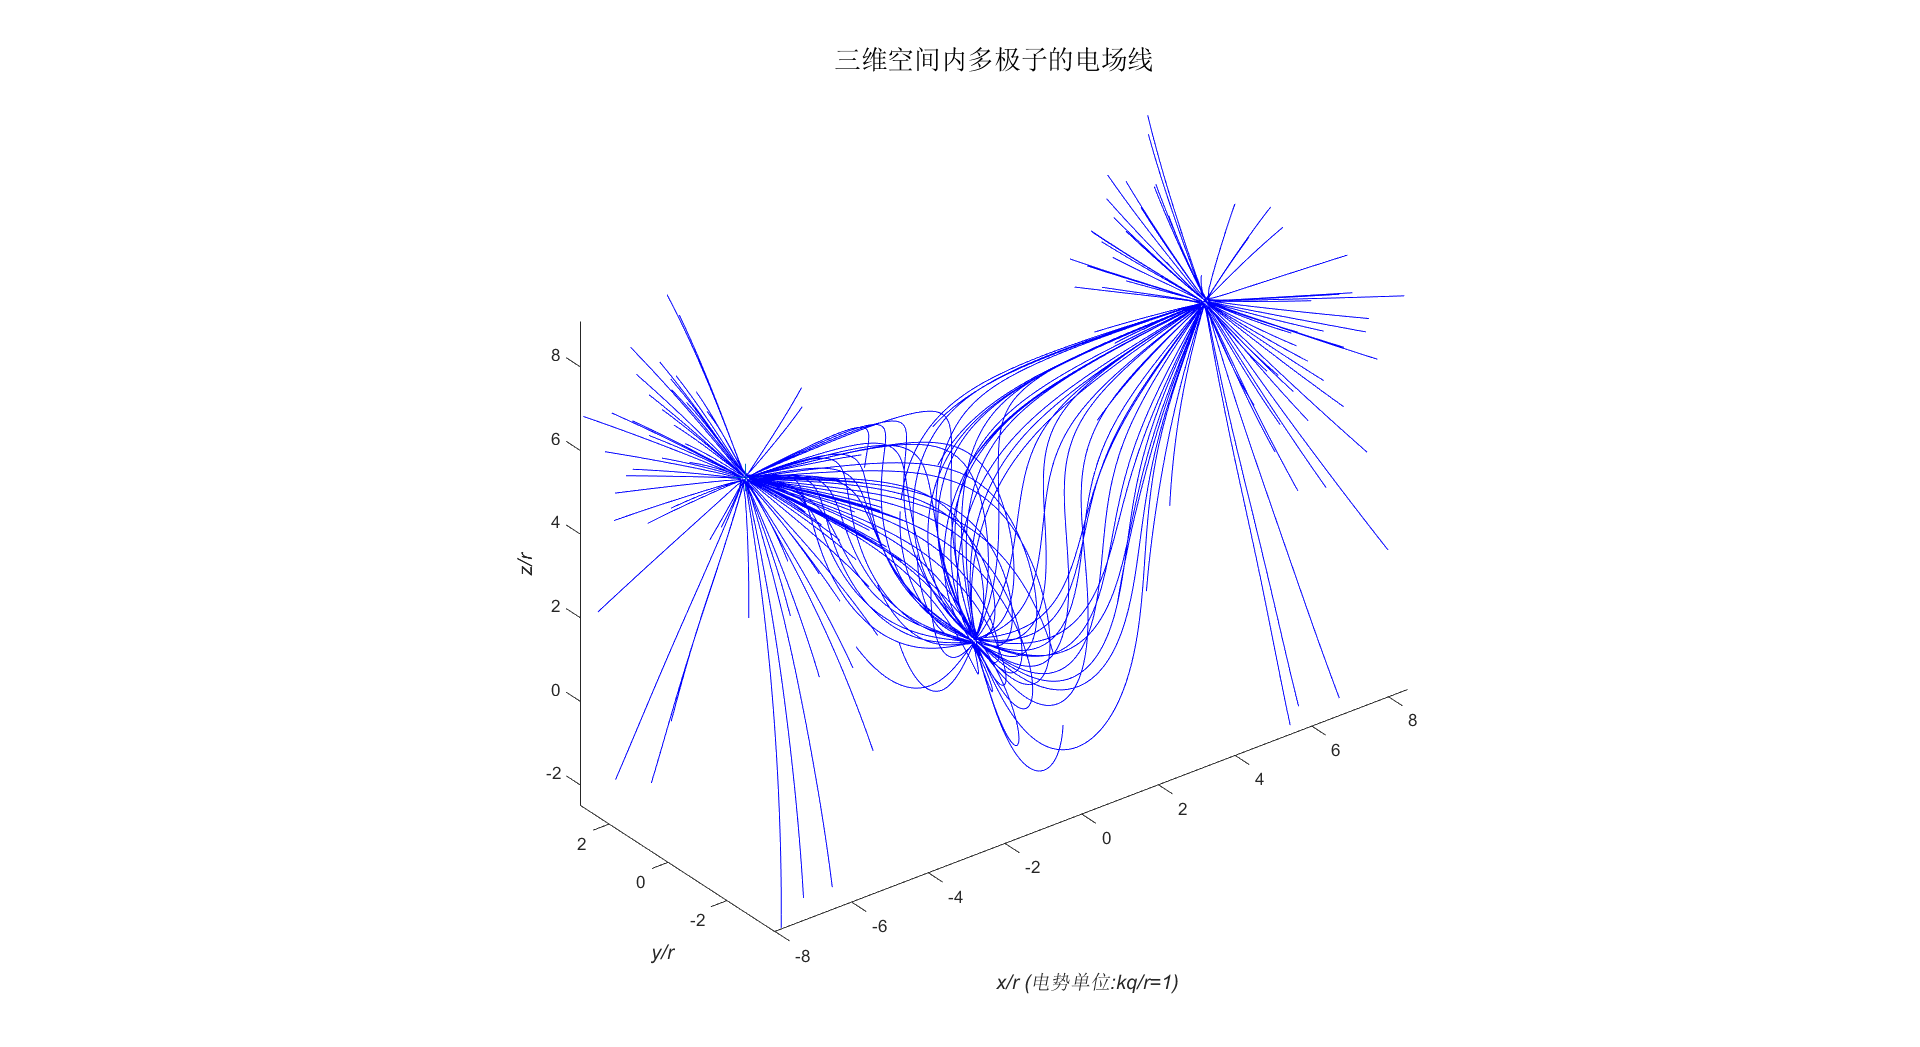
\includegraphics[scale=0.15]{测试5.png}
	\end{figure}
	\begin{figure}[H]
		\centering
		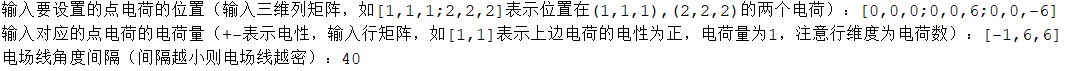
\includegraphics[scale=0.4]{ceshi6.png}
	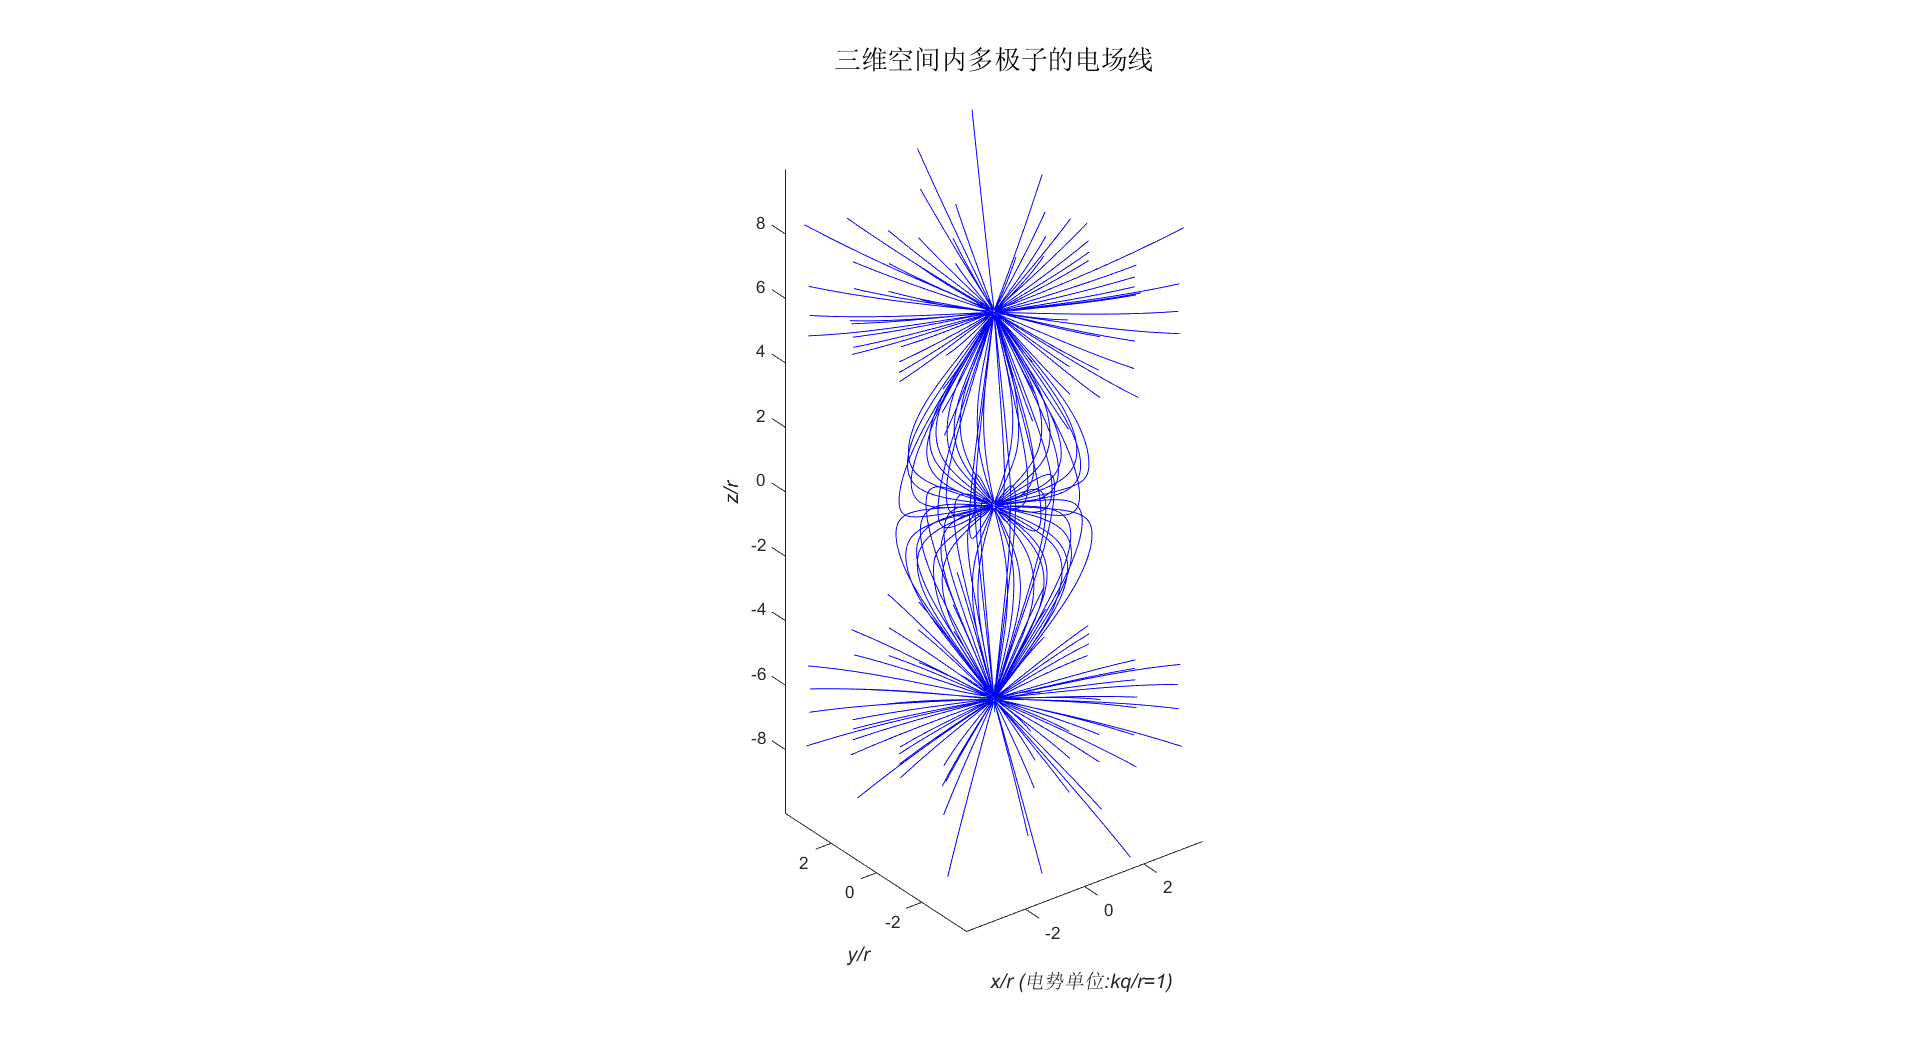
\includegraphics[scale=0.15]{测试6.png}
	\end{figure}
    \section{结论}
    \par 本次论文研究深入探索了MATLAB语言,并对电磁学知识进行整合提炼,主要研究了几个在做题时经常碰到的物理模型,并成功地运用MATLAB语言进行了可视化展示。
    \par 在研究过程中,不仅复习了电磁学知识,还学会了如何利用MATLAB语言进行电磁学模型的可视化。通过绘制图像和分析数据,成功地展示了各个模型的特性和规律。这不仅加深了我对电磁学原理和现象的理解,还让我领略到了自然之美。
    \par 通过运用MATLAB对电场、磁场等进行仿真,能够直观地观察到它们的分布和变化规律。通过绘制电场线、等势线、磁感应线等图像,可以得出了更深入的结论,并能够将其可视化呈现。这使我更好地理解了电磁学的重要概念和数学模型。
    \par 尽管我的知识积累还不够丰富,一些高级功能尚未实现,但我对进一步深入学习和完善这些模型充满期待。
    \par 这次研究给我带来了很多收获,激发了我对电磁学领域的兴趣和热情。我相信在更深入的学习和实践中,我将能够进一步提升自己的能力,并实现更多高级功能。我会继续努力学习,以便更好地理解和应用电磁学知识,并为未来的研究和工作做好准备。
    \par 附上我的GitH网页网址:\href{https://github.com/chenxinqi041027/chenxinqi041027.github.io}{My GitHub Website}
\end{multicols}
\renewcommand\refname{参考文献}
\bibliographystyle{unsrt}
\bibliography{陈昕琪_Pb22111711.bib}
\par [1]电磁学 中国科学技术大学交叉学科基础物理教程(第2版) 叶邦角 中国科学技术大学 2018
\par [2]林春丹,等.基于Matlab的静电场可视化教学示例[J].大学物理实验,2018, 31(3).
\par [3]金华.静电场线描绘实验的Matlab辅助教学[J].科技风,2018(34).
\par [4]高翠云,汪莉丽.利用 MATLAB 进行电磁学计算及可视 化教学.电气电子教学学报,2006(2);90~92
\par [5]蒋志洁,阳生红,张曰理. 运用 Matlab GUI 辅助大学 物理实验[J]. 物理实验,2017(6) :23-27.
\par [6]钟季康,鲍鸿吉.大学物理习题计算机解法---MATLAB编程应用[M].北京:机械工业出版社
\end{document}